\documentclass[a4paper, 12pt, master, utf8]{etf}

\usepackage[a4paper, margin=25mm]{geometry}
\usepackage{gentium} % font
\usepackage{enumitem}
\usepackage[linesnumbered, algoruled, longend]{algorithm2e} % za pseudo kod
\usepackage{rotating} % za sidetable

\usepackage{pgfplots}
\usepackage{tikz}
\usepackage{pgf-umlcd}

\usepackage{algpseudocode}

\addto\extrasserbianc{\def\bibname{Литература}\let\refname\bibname}
\SetAlgorithmName{Псеудо код}{псеудо код}{Листа псеудо кодова}
\SetInd{2mm}{3mm} % za pseudo kod razmak pre i posle
\newcommand*\rot{\rotatebox{90}} % za rotirane labele tabele

\author{Алекса Рачић}
\date{\today}
\title{Анализа проблема апстрактног резоновања у неуронским мрежама на примеру Рејвенових матрица}
\indeks{2019/0728}
\mentor{доц др. Марко Мишић}
\usepackage{array}
\newcolumntype{P}[1]{>{\centering\arraybackslash}p{#1}}
\usepackage{titlesec}
\usepackage{setspace}
\usepackage[flushleft]{threeparttable}

\titleformat{\chapter}[display]
  {\normalfont\bfseries}{}{0pt}{\Huge}

\begin{document}

\maketitle

\tableofcontents

\addtocontents{toc}{\protect\thispagestyle{empty}}
\pagenumbering{arabic}
\onehalfspacing
\newpage

\chapter{Увод}
\label{sec:1}

Главни циљ у домену вештачке интелигенције и машинског учења јесте стварање машине која ће имати когнитивне способности које су исте или боље од човека. Ово подразумева да машина мора бити способна да учи, закључује, решава проблеме и да се адаптира на нове ситуације, односно да поседује своју интелигенцију.
Једна од фудаменталних карактеристика људске интелигенције је апстрактно закључивање - способност разазнавања шаблона, извођења закључака и решавања проблема у доменима који превазилазе просто меморисање података.
\newline

У том контексту, високо цењена Рејвенова серија тестова, коју је представио Џон Рејвен у својем раду из 1938. године \cite{raven1938raven}, представља главни инструмент у процени апстрактног закључивања. Ови тестови се заснивају на употреби апстрактних визуелних стимула у облику матрица, 
помоћу којих се испитује способност посматрача да идентификује скривене образце и закључи о правилности или тенденцијама. Успешно решавање ових матрица захтева способност апстрактног и логичког закључивања, што га чини изазовним мерилом за анализу и процену когнитивних способности како људи, тако и алгоритама у области вештачке интелигенције.
\newline 

Најчешћи облик Рејвеновоф теста се састоји од 3x3 матрице која садржи 8 познатих композиција и један непознати образац у доњем десном углу. Посматрач треба да одабере један од 8 понуђених одговора који најбоље одговара непознатом обрасцу. Постоји више различитих варијанти Рејвенових матрица, али је њихова основна идеја иста. На слици \ref{fig:raven_example} 
је приказан пример једне од варијанти Рејвенових матрица која ће се користити за анализу у овом раду.
\newline

\begin{figure}[h]
    \centering
    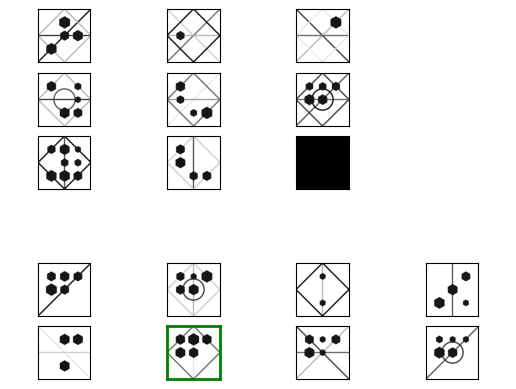
\includegraphics[width=0.7\textwidth]{images/output.png}
    \caption{Пример Рејвенове матрице.}
    \label{fig:raven_example}
\end{figure}

Поставља се питање: Да ли тестови интелигенције могу дати увид у интелигенцију машине? На крају 
крајева, машина се учи на конкретном домену задатака, док је људска интелигенција општег карактера. 
Али, чак и у случају људи, вежбом се могу пронаћи хеуристике које помажу у решавању таквих текстова као 
што је доказано у раду где су тренингом успели да повећају резултате испитаника на тестовима интелигенције \cite{te2001practice}.
\newline

Упркос томе, у овом раду се сматра да решавање Рејвенових матрица неуронским мрежама може да пружи увид у њихову интелигенцију и моћ апстрактног резоновања. 
\newline

У сврху анализе изабране су три различите архитектуре неуронских мрежа, које су обучаване на примерима Рејвенових тестова како би добили увид у њихову способност апстрактног закључивања.
Поред тога, у раду је представљен и софтверски оквир који је коришћен за имплементацију и тренирање неуронских мрежа, као и за тестирање и анализу резултата. 

\chapter{О проблему}
\label{sec:2}

Главни изазов представља сама детекција облика и линија на слици. Потребно је пројектовати архитектуру неуронске мреже која је у стању да разуме облике
са слике као и њихое односе. Такође је потрено да науронска мрежа донесе одлуку који од понуђених одговора најбоље одговара непознатом обрасцу.
\newline

Изабрану архитектуру је потребно моделовати операцијама над скупом података како би рачунар могао да је извршава. Потребно је применити алгоритме учења неуронским мрежа пазећи на њихвоу ефикасност у извршавању.
\newline

На крају је потребан софтверски оквир који ће омогућити тренирање и тестирање неуронских мрежа, као и анализу резултата. 
Оквир треба да буде једноставан за коришћење и да омогући лаку модификацију архитектуре неуронске 
мреже. Такође, треба да садржи механизме за обучавање неуралне мреже, односно нашег модела. Његово тестирање на различитим скупом података и 
резултате визуелно прикаже како би били разумљиви човеку.

\section{Формулација проблема}
\label{sec:21}
Проблем којим се овај рад бави је обиман, али се може дефинисати следећим скупом задатака:

\begin{itemize}[noitemsep]
    \item  Пројектовање адекватне архитектуре неуронске мреже за решавање Рејвенових матрица,
    \item  Моделовање неуронске мреже помоћу софтверског оквира,
    \item  Тренирање неуронске мреже на скупу података,
    \item  Тестирање неуронске мреже на скупу података,
    \item  Анализа резултата и унапређење модела.
\end{itemize}

\section{Машинско учење}
\label{sec:22}
Машинско учење представља процес учења модела из података са циљем постављања параметара тог модела 
на оптималне вредности. Циљ је да се модел обучи да даје најбоље резултате на скупу података који му 
су доступни. Ово се постиже минимизацијом функције губитка (енг. \textit{loss function}). 
Функција губитка је кључни аспект у машинском учењу и она оцењује колико добро модел класификује 
или предвиђа резултате на основу улазних података. Што је вредност функције губитка мања, то је модел бољи у свом задатку. 
Процес учења модела своди се на постављање параметара модела тако да се 
вредност функције губитка минимизује, односно да модел тачније предвиђа жељене резултате. 
Ова оптимизација параметара модела је срж машинског учења и она омогућава моделима да постану 
способни за различите задатке и анализе на основу доступних података. 
У овом раду ћемо користити надгледано учење где
за сваки улаз имамо јасно дефинисане излазе које очекујемо од нашег модела.
\newline

Стога да би се успешно обучила машина потребни су: модел, алгоритам за промену параметара модела (оптимизатор), функција губитка и скуп података.

\section{Скуп података}
\label{sec:23}
У циљу што бољег обучавања неуронске мреже потребно је да се користи што већи скуп података. 
Даље, потребно је да подаци буду раздвојени у скуп за тренинг, валидацију и тестирање како би се евалуација 
модела радила на невиђеним подацима. У овом раду је коришћен скуп урађених Рејвенових тестова
који је представљен у раду \cite{barrett_measuring_2018}. Метода којом су креирани тестови се састоји из следећих корака.
\newline

Прво се дефинише скуп типова релација, типова објеката и типова атрибута који ће се користити у генерисању тестова. Релације представљају однос у којим се облици или линије налазе у једном реду или колони. 
Облик се односи на то да ли се релација примењује на линије у позадини или облике који се налазе на композицијама, а тип атрибута се односи на то шта се мења у прогресији.
У референтном раду су коришћени следећи скупови:

\begin{itemize}[noitemsep]
    \item  \textbf{Тип релације ($\mathrm{P}$)}: прогресија (енг. \textit{progression}), ексклузивно ИЛИ (енг. \textit{XOR}), ИЛИ (енг. \textit{OR}), И (енг. \textit{AND}), козистентна унија, (енг. \textit{consistent union}),
    \item  \textbf{Тип објекта ($\mathrm{O}$)}: облик (енг. \textit{shape}), линија (енг. \textit{line}),
    \item  \textbf{Тип атрибута ($\mathrm{A}$)}: величина (енг. \textit{size}), тип (енг. \textit{type}), боја (енг. \textit{colour}), позиција (енг. \textit{position}), број (енг. \textit{number}).
\end{itemize}

Затим се прави скуп тројки $S = \{[p, o, a]: p \in P, i \in O, a \in A\}$ . У референтном раду је величина скупа ограничена на мексимално четири тројке.
Сваки скуп дефинише један тест пример.
\newline

После тога се насумично бирају остали атрибути ($\mathrm{A}$). Током овог процеса је праћено да новододељени насумични атрибути не чине нови скуп тројки. У случају да није могуће изабрати такав атрибут сваки објекат у матрици узима исту вредност датог атрибута. 
\newline

Слике које нису тачни одговори се генеришу насумично.
\newline

На основу тројки и атрибута се креирају слике Рејвенових матрица као и потенцијални одговори.
\newline

На примеру \ref{fig:raven_example} су присутне тројке: ['или', 'облик', 'позиција'], ['или', 'линија', 'тип']. Прва тројка диригује да у једној колони позиције облика у последњем реду морају бити логичко или позиција у прва два реда. Док  се друга тројка односи на то да у једном реду у последњој колони морају да се
нађу сви облици линија као у прве две колоне. На основу наведеног је тачан одговор композиција под редним бројем 6.
\newline

Аутори референтног рада су представили осам различитих скупова података код којих се разликује заступљеност тројки као и вредности који атрибути могу имати и њихова заступљеност у скупу за тренирање и тестирање. 
\newline

Скуп података је доступан јавности и у овом раду је коришћен готов скуп података \cite{noauthor_procedurally_2023}.
Изабран је неутрални (енг. \textit{neutral}) скуп података где су све тројке једнако заступљене у скупу за тренирање, валидацију и тестирање. 
\newline

Скуп садржи 1.42 милиона Рејвенових тестова различите тежине подељених у три подскупа. Тренинг скуп садржи 1.2 милина, скуп за тестирање 400 хиљада, а скуп за валидацију 20 хиљада примера. Подаци су у \textit{.npz} формату.
Свака датотека садржи следеће информације:

\begin{itemize}[noitemsep]
    \item \textbf{Слика (енг. \textit{image})}: 160x160x16 матрица са вредностима од 0 до 255 која представља 16 црнобелих слика. Првих 8 слика представљају контекст Рејвенове матрице, а последњих осам потенцијалне одговоре,
    \item \textbf{Тројке (енг. \textit{meta\_target})}: Скуп тројки $\{[p, o, a]: p \in P, i \in O, a \in A\}$ који су присутни у примеру, 
    \item \textbf{Тачан одговор (енг. \textit{target})}: Реди број тачног одговора.
\end{itemize}



\section{Неуронске мреже}
\label{sec:23}

У контексту неуронских мрежа, неурон представља основну јединицу обраде информација. 
Он симулира рад људског неурона у мозгу. Графички изглед једног неурона је приказана на слици \ref{fig:neuron}. Сваки неурон прима улазне сигнале $x_0, x_1 ... x_N$, обрађује их, и издаје излазни сигнал $y$. 
\newline

Тежине (енг. \textit{weights}) $w_0, w_1 ... w_N$ представљају параметре који се користе за модификацију улазних података прослеђених неурону. Сваки улаз у неурон је помножен са одговарајућом тежином. Тежине утичу на значајност улазних података и одређују њихову улогу у 
формирању излаза неурона. Процес учења у neuronskim мрежама, познат као обука, састоји се из ажурирања и промене тежина како би мрежа најбоље моделовала жељени задатак.
\newline

Збир улаза помноженим са тежинама сигнала се прослеђује активационој функцији $f$. 
Коришћењем активационих функција, неуронске мреже су у могућности да моделирају нетривијалне односе између улазних и излазних података. Овај излазни сигнал затим служи као улаз за следећи слој неурона у мрежи.
\newline

Пристрасност (енг. \textit{bias}) је додатни параметар који се користи за прилагођавање излаза неурона. Тежина којом пристрасност утиче на актиациону функцију је одређена тежином $b$.
\newline

\begin{figure}[h]
    \centering
    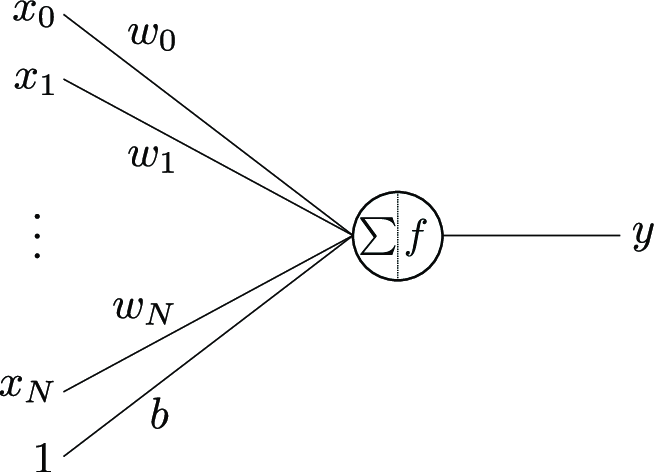
\includegraphics[width=0.7\textwidth]{images/neuron.png}
    \caption{Графички приказ једног неурона. \cite{ioannou_structural_2017}}
    \label{fig:neuron}
\end{figure}

Математички израз како тежине, улази и пристрасност утичу на излазни сигнал је дат једначином \ref{eq:neuron}.
\newline

\begin{equation}
    y = f\left(\sum_{i=1}^{n} w_i x_i + b\right)
    \label{eq:neuron}
\end{equation}
\subsection{Потпуно повезане неуронске мреже}
\label{sec:232}

Потпуно повезане неуронске мреже (ППНМ) (енг. Fully Connected Neural Networks) су скуп повезаних неурона описаних у \ref{sec:23}. Састоји се од више слојева, први слој се назива улазни слој,
а последњи слој се назива излазни слој. Сви остали слојеви се називају скривени слојеви (енг. \textit{hidden layer}). На слици \ref{fig:fc} је графички приказана неуронска мрежа која има 2 скривена слоја.
Сваки слој може да има произвољан број неурона, а неуронска мрежа може да има произвољан број скривених слојева. Мењајући архитектуру, односно број неурона у једном слоју и број слојева
се мења моћ мреже и комплексност задатка који мрежа може да решава.


\begin{figure}[h]
    \centering
    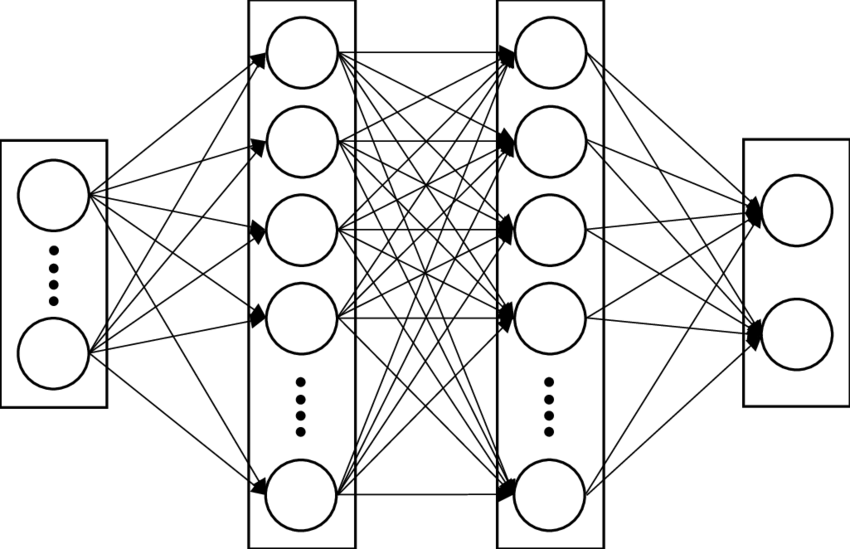
\includegraphics[width=0.7\textwidth]{images/fc.png}
    \caption{Графички приказ потпуно повезане неуралне мреже. \cite{anwar_learned_2017}}
    \label{fig:fc}
\end{figure}


ППНМ прима само децималне бројеве као улаз и битно је да приликом тренирања и предикције да исти вредности атрибута улазних података улазе у потпуно повезану мрежу на исти улаз.
Овакав тип мреже се најбоље показао на проблемима класификације \cite{noauthor_artificial_2023}.

\subsection{Конволуционе неуронске мреже}
\label{sec:232}

Конволуциона неуронска мрежа (КНМ) (енгл. Convolutional Neural Network - CNN) представља подврсту дубоких неуронских мрежа 
која је развијена за обраду и анализу података, као што су слике и видео записи. Главна одлика ове врсте неуронске мреже јесу конволуциони слојеви који примењују велик број 
филтара на улазну слику. На графичком приказу \ref{fig:convolution} операције конволуције I представља улаз, а К филтар, који се помера кроз улаз и множи са суседним вредностима улазне слике. Током процеса тренирања 
филтри мењају своје вредности и понашају се као тежине. Могуће је на исти слику примењивати већи број филтера и то се означава као број канала. Поред тога конволуционе слојеве дефинише померај који говори за који број пиксела се филтар помера приликом конволуције.

\begin{figure}[h]
    \centering
    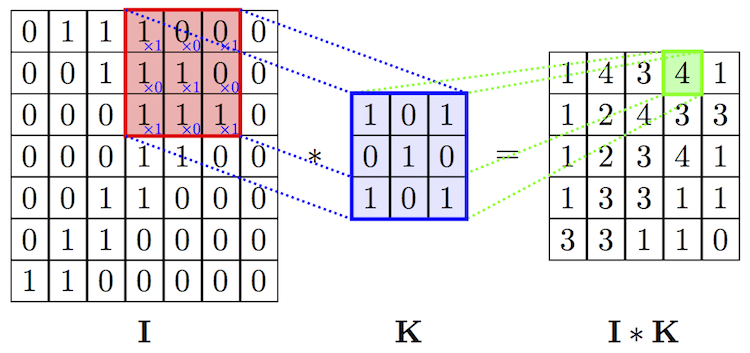
\includegraphics[width=0.7\textwidth]{images/convolution.png}
    \caption{Графички приказ конволуције. \cite{s_mohamed_detection_2017}}
    \label{fig:convolution}
\end{figure}

Математички приказ \ref{eq:con} конволуције где М и Н представљају висину и ширину филтера.

\begin{equation}
    (I * K)[i, j] = \sum_{m=0}^{M-1} \sum_{n=0}^{N-1} I[m, n] \cdot I[i-m, j-n]
    \label{eq:con}
\end{equation}

Конволуциони слојеви се не могу сами тренирати и обично су праћени слојевима неуралне мреже који раде класификацију.
Стога се архитектура Конволуционе неуралне мреже \ref{fig:cnn} се састоји од низа конволуционих слојева праћеним неким другим типом неуралне мреже, обично је то потпуно повезана мрежа из \ref{sec:232} .

\begin{figure}[h]
    \centering
    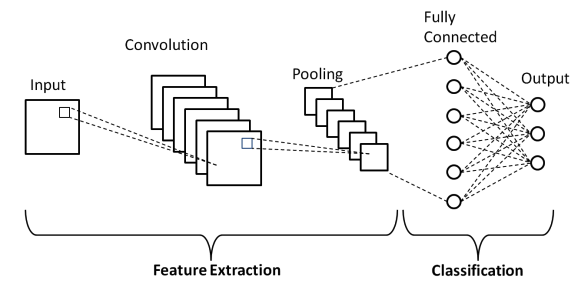
\includegraphics[width=0.7\textwidth]{images/cnn.png}
    \caption{Графички приказ архитектуре конволуционе неуронске мреже. \cite{s_mohamed_detection_2017}}
    \label{fig:cnn}
\end{figure}

Класификациони слој служи да се декодује апстрактни запис слике из латентног вектора и квантификује излаз конволуционих слојева како би функција губитка могла оценити
грешку мреже приликом тренирања.

\subsection{Рекурентне неуронске мреже}
\label{sec:233}

Рекурентне неуронске мреже (РНМ) (енг. Recurrent Neural Networks - RNN) представљају тип неуронских мрежа које су дизајниране за обраду и анализу 
серијских, узајамно зависних података, као што су текст, временске серије и генетички подаци. На слици \ref{fig:rnn} је приказан изглед
једног неурона у рекурентној неуронској мрежи. На левој страни слике је приказан графички изглед неурона $h^{1}_1$. Излаз неурона се враћа на улаз са одређеном тежином.
Ово значи да следећи излаз неурона зависи од претходног излаза. Ако развојемо неурон кроз време (слика \ref*{fig:rnn} десно), приметимо да ће на излаз $y_T$ утицати
улази $x_1 , x_t, x_T$.

\begin{figure}[h]
    \centering
    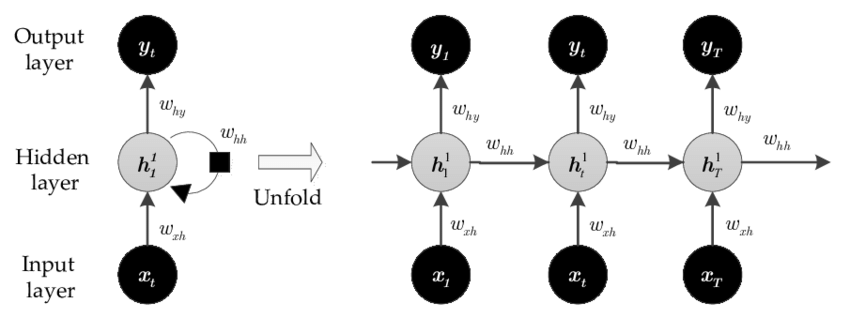
\includegraphics[width=0.7\textwidth]{images/rnn.png}
    \caption{Графички приказ једног неурона РНМ. \cite{husein_day-ahead_2019}}
    \label{fig:rnn}
\end{figure}

\subsubsection{Неуронске мреже са краткорочном и дугорочном меморијом}

Неуронске мреже са краткорочном и дугорочном меморијом (КДМ) (енг. Long Short Term Memory - LSTM) је специфичан тип рекурентне невралне мреже (РНМ).
Онa је дизајнирана да реши проблем нестанка градијента \footnote{Проблем нестанка градијента је случај када, током обучавања мреже, се градијенти значајно смањи при сваком обрадном слоју.} (енг. vanishing gradient) и 
екплодирајућих градијената (енг. exploding gradient)\footnote{Проблем експлодирајућих градијента је случај када, током обучавања мреже, се градијенти значајно повећају при сваком обрадном слоју.} који се често јавља код стандардних РНМ-ова.
Ови проблеми доводе до нестабилности мреже и прекорачења рачунарског ограничења за величине градијената.
\newline

\begin{figure}[h]
    \centering
    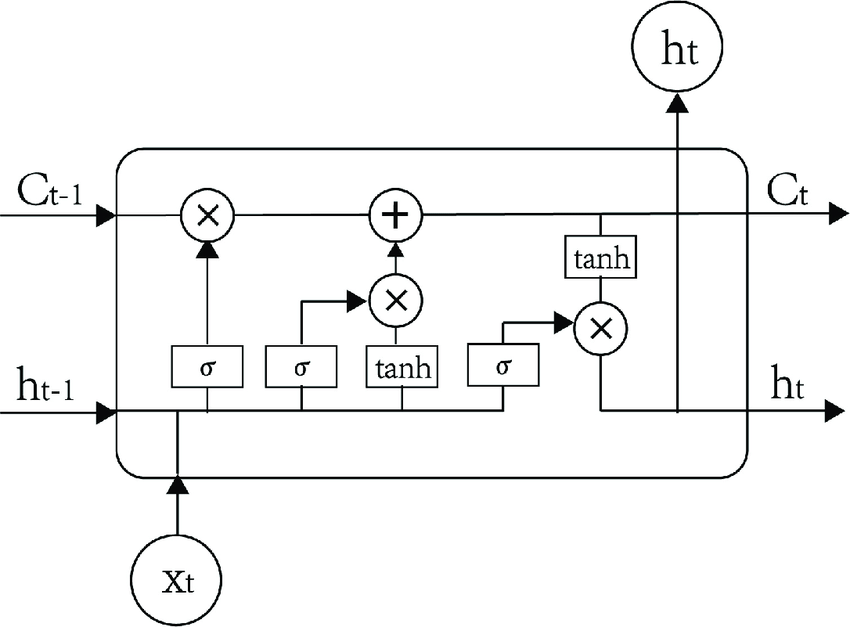
\includegraphics[width=0.7\textwidth]{images/LSTM.png}
    \caption{Графички приказ једног КДМ блока. \cite{qiu_forecasting_2020}}
    \label{fig:LSTM}
\end{figure}

На слици \ref{fig:LSTM} је приказан изглед једног КДМ блока. Блок има три улаза. Улаз за сигнал дугорочне меморије ($C_{t-1}$), краткорочне меморије($h_{t-1}$) и улаз новог сигнала ($X_t$). Такође има два излаза који представњају нову информацију краткорочне и дугорочне меморије.
Блокови се серијски повезују како би се радила предикција серија. КДМ блок садржи 3 капије, пратећи са лева на десно са слике \ref{fig:LSTM}:

\begin{itemize}[noitemsep]
    \item \textbf{Капија за заборавњање (енг. Forget Gate)}: Ова капија одређује који део дугорочне меморије ће да се заборави.
    \item \textbf{Капија за ажуриранје (енг. Update Gate)}: Ова капија одређује колико ће дугорочну меморију да ажурира новим информацијама.
    \item  \textbf{Капија за излаз (енг. Output Gate)}: Ова капија одређује који део интерне меморије треба да буде излаз.
\end{itemize}

Блок садржи више активационих функција које регулишу сваку капију. Активациона функција хиперболичког тангенса ($tanh$) и сигмоидна функција ($\sigma$) ће бити детаљније описане у секцији о активационим функцијама \ref{sec:24}.

\subsection{Релационе неуронске мреже}
\label{sec:234}
Релациона неуронска мрежа (РНН) (енг. Relational Neural Network - RNN) су дизајниране да обраде информације које се односе на релације између објеката у систему. За неки сет улаза могу да одреде у каквој су улази релацији.
То се постиже тако што два различита улаза пропустимо кроз посебне неуронске мреже, излазе спојимо, а затим опет пропустимо кроз следећу неуралну мрежу.


\section{Активационе Функције}
\label{sec:24}
Активационе функције су математичке функције које се користе у неуронским мрежама да би се одређивала активација (излаз) 
неурона на основу његових улаза. Активационе функције доприносе нелинеарности у моделима, што је битно за то да мрежа може да апроксимира комплексне функције.

\subsection{Функција активације исправљача}
\label{sec:241}

Функција активације исправљача (енг.  ReLU - Rectified Linear Unit) активациона функција дефинисана као позитиван део свог аргумента. Све вредности које су мање 
од нуле постају нула, а веће се не мењају. Функција у математичком облику је дата изразом \ref{eq:ReLu}, a њен графички изглед је приказан на слици \ref{fig:relu}.

\begin{equation}
    f(x) = \max(0, x)
    \label{eq:ReLu}
\end{equation}

\begin{figure}[h]
    \centering
    \begin{tikzpicture}
        \begin{axis}[
            xlabel=$x$,
            ylabel=$\text{ReLu}(x)$,
            ymin=-1, ymax=3,
            xmin=-1, xmax=2,
            axis lines=middle,
            axis line style={->},
            samples=400
        ]
        \addplot[domain=-1:0,blue,thick] {0};
        \addplot[domain=0:2,blue,thick] {x};
        \end{axis}
        \end{tikzpicture}
    \caption{Графички приказ функције активације исправљача}
    \label{fig:relu}
\end{figure}

Ова функција има проблем са мртвим неуронима, што су неурони који се никада не активирају за одређене улазне вредности. 
Ово може довести до тога да ти неурони не допринесу тренингу и остану неактивни.

\subsection{Хиперболички тангенс}
\label{sec:242}
Хиперболички тангенс, обично означен као tanh, је активациона функција која све излазне вредности скупља у опсег $[-1, 1]$.
Функција у математичком облику је дата изразом \ref{eq:tanh}, a њен графички изглед је приказан на слици \ref{fig:tanh}.

\begin{equation}
    f(x) = \frac{e^{x} - e^{-x}}{e^{x} + e^{-x}}
    \label{eq:tanh}
\end{equation}

\begin{figure}[h]
    \centering
    \begin{tikzpicture}
        \begin{axis}[
            xlabel=$x$,
            ylabel=$\tanh(x)$,
            ymin=-1.2, ymax=1.2,
            xmin=-3, xmax=3,
            axis lines=middle,
            axis line style={->},
            samples=200
        ]
        \addplot[domain=-3:3,blue,thick] {tanh(x)};
    \end{axis}
    \end{tikzpicture}
    \caption{Графички приказ функције активације хиперболичког тангенса}
    \label{fig:tanh}
\end{figure}

\subsection{Сигмоидна функција}
\label{sec:243}
сигмоидна функција активације јематематичка функција која има карактеристичну криву у облику латиничног слова „S” или сигмоидну криву.
Означава се грчким словом сигма $\sigma$. По облику је слична хиперболичном тангенсу, али се разликује у томе што скупља вредности у опсег $[0,1]$ и центрирана је око вредности 0.5.
Функција у математичком облику је дата изразом \ref{eq:sigmoid}, a њен графички изглед је приказан на слици \ref{fig:sigmoid}.

\begin{equation}
    f(x) = \frac{1}{1 + e^{-x}}
    \label{eq:sigmoid}
\end{equation}

\begin{figure}[h]
    \centering
    \begin{tikzpicture}
        \begin{axis}[
            xlabel=$x$,
            ylabel=$\sigma(x)$,
            ymin=0, ymax=1,
            xmin=-5, xmax=5,
            axis lines=middle,
            axis line style={->},
            samples=200
        ]
        \addplot[domain=-5:5,blue,thick] {1/(1 + exp(-x))};
        \end{axis}
        \end{tikzpicture}
    \caption{Графички приказ функције активације сигмоидне функције}
    \label{fig:sigmoid}
\end{figure}

\section{Функције грешке}
\label{sec:25}

Функција грешке (енг. loss function или error function) оцењује колико су предвиђени резултати (излази) различити од стварних резултата (циљне вредности) и представља вредност коју алгоритам 
оптимизације покушава да минимизује током тренинга модела.

\subsection{Унакрсна ентропија}
\label{sec:261}

Унакрсна ентропија (енг. Cross-Entropy Loss) је функција грешке која се често користи у задацима класификације. 
Ова функција се користи за мерење разлике између стварних и предвиђених вероватноћа класификације.

Нека имамо $C$ класа у проблему класификације, где свака класа има своју стварну вероватноћу $p_i$ и предвиђену вероватноћу $q_i$ (где $i$ означава индекс класе).
\newline 

Унакрсна ентропија између стварних и предвиђених вероватноћа се израчунава помоћу израза \ref{eq:loss}.


\begin{equation}
    \label{eq:loss}
    H(p, q) = -\sum_{i=1}^{C} p_i \log(q_i)
\end{equation}
\section{Оптимизатори модела}
\label{sec:26}

Оптимизатори представљају алгоритме и методе који се користе за ажурирање параметара модела са циљем минимизовања функције грешке.
Први корак представња израчунавање градијента сваког неурона. Градијент се рачуна по следећем алгоритму:

\begin{enumerate}
    \item Улаз се пропусти кроз неуралну мрежу (енг. \textit{Forward Pass}),
    \item Израчуна се грешка модела у односу на очекивани излаз,
    \item За сваки неурон се рачуна градијент функције грешке у односу на излаз тог слоја применом ланчаног правила извода (енг. \textit{Backpropagation}).
\end{enumerate}

\subsection{Стохастички спуст (\textit{Stochastic gradient descent - SGD})}

Алгоритам стохастичког спуста низ градијенте (енг. \textit{Stochastic gradient descent - SGD}) је алгоритам који на основу израчунатих градијената мења вредности тежина у смеру смањења функције грешке.
Понашање алгоритма је условњено параметром стопе учења (енг. \textit{leraning rate}) који одређује за који проценат градијента желимо да променимо тежине модела.
Алгоритма је приказан у псеудо коду \ref{alg1}.
\newline

\begin{algorithm}
    \label{alg1}
    \DontPrintSemicolon
    \For{$epoch \gets 1$ \KwTo $N$} {
        \For{$batch \gets 1$ \KwTo $num\_batches$} {
            $gradient = compute\_gradient(data, model)$ \;
            $model\_parameters = model\_parameters - learning\_rate \cdot gradient$ \;
        }
    }
    \caption{Главна петља са SGD оптимизатором}
\end{algorithm}

Стохастички спуст низ градијенте може бити нестабилан током оптимизације. Градијенти се израчунавају за сваки мини-батч, ажурирања тежина су стохастичка и често се манифестују као шум у конвергенцији. Ово може резултовати осцилацијама или споријим конвергенцијама.

Такође је подложан заглављивању у локалним минимумима функције грешке. Ако је стопа учења превелика, алгоритам може скакати преко минимума, док ће са премалом стопом учења конвергенција бити спора или уопште не конвергирати.
\newline

\subsection{Адам (\textit{\textit{Adaptive Moment Estimation - Adam}})}

Аутори рада \cite{kingma_adam_2017} су представили модификацију на стохастички спуст - АДАМ (енг. \textit{Adaptive Moment Estimation - ADAM }).
Адам адаптивно регулише стопу учења за сваки параметар модела. Ово значи да се стопа учења аутоматски прилагођава за сваки параметар на основу историје градијената.
Он користи механизам моментума како би убрзао и стабилизовао процес оптимизације. Моментум омогућава алгоритму да пређе платое и избегне локалне минимуме.
Алгоритам, поред параметра стопе учења, уводи и следеће параметре:

\begin{itemize}
    \item \textbf{$\beta1$} - у којој мери први моментум утиче на стопу учења,
    \item \textbf{$\beta2$} - У којој мери други моментум утиче на стопу учења,
    \item \textbf{$\epsilon$} - Мала вредност која спречава дељење са нулом.
\end{itemize}

Алгоритам за Адам је приказан у псеудокоду \ref{alg2} .

\begin{algorithm}[H]
    \label{alg2}
    \DontPrintSemicolon
    \For{$epoch \gets 1$ \KwTo $N$} {
        \For{$batch \gets 1$ \KwTo $num\_batches$} {
            $gradient = compute\_gradient(data, model)$ \;
            $m \gets \beta1 \cdot m + (1 - \beta1) \cdot gradient$ \;
            $v \gets \beta2 \cdot v + (1 - \beta2) \cdot (gradient \cdot gradient)$ \;
            $m_{\text{corrected}} \gets \frac{m}{1 - \beta1^t}$ \;
            $v_{\text{corrected}} \gets \frac{v}{1 - \beta2^t}$ \;
            $model\_parameters = model\_parameters - \frac{learning\_rate \cdot m_{\text{corrected}}}{\sqrt{v_{\text{corrected}}} + \epsilon}$ \;
        }
    }
    \caption{Главна петља са Adam оптимизатором}
\end{algorithm}

\section{Технике регуларизације и убрзавања конвергенције}
\label{sec:28}
Технике регуларизације служе како би умањили ефекат преобучавања\footnote{Појава када се модел превише прилагоди скупу података за тренирање}. Са друге стране 
подаци који се користе за обучавање могу да имају аутлајере који негативно утичу на конвергенцију тренинга.

\subsection{Изоставњање неурона (\textit{Dropout})}

Дропоут (енг. \textit{Dropout}) слој се користи како би у процесу тренирања прескочили ажурирање тежина одређеног процента неурона у слоју где користимо ову технику.
Он делује као регуларизација јер спречава да се било који појединачни неурон или група неурона превише ослања на одређене карактеристике у скупу за тренирање.
Ово резултује у смањењу преобучавања и доприноси бољој генерализацији. 

\subsection{Нормализација гомиле (\textit{Batch Normalization})}

Нормализација гомиле (енг. \textit{Batch Normalization}) је техника која се користи да би се побољшала стабилност тренирања и убрзао процес конвергенције у дубоким неуронским мрежама. 
Током тренирања, ова техника нормализује активације сваког слоја тако да имају стандардну средњу вредност и варијансу у оквиру сваке гомиле.
На овај начин се уањује утицај аутлајера и доприности стабилности учења.


\section{Додатнe функције и слојеви}
\label{sec:26}

\subsection{Софтмакс (\textit{softmax})}

Софтмакс функција се често користи у неуралним мрежама за решавање задатака класификације, као и за генерисање расподеле вероватноћа излаза из мреже. 
Она трансформише илаз тако да све вредности излаза леже у интервалу између 0 и 1 и да се сума свих вредности излаза једнака 1 
Формално, софтмакс функција је дефинисана у изразу \ref{eq:ss} за вектор излаза Z :

\begin{equation}
    \label{eq:ss}
    \text{softmax}(z)_i = \frac{e^{z_i}}{\sum_{j=1}^{N} e^{z_j}}
\end{equation}

Где:

\begin{itemize}
    \item z је вектор излаза модела за сваку од N класа.
    \item e представља експоненцијалну функцију (елемент по елемент).
    \item i је индекс класе за коју рачунамо вероватноћу.
\end{itemize}


\subsection{Функција највећег аргумента (\textit{argmax})}
Фунција највећег аргумента враћа позицију највећег елемента из вектора вредности.

\chapter{Коришћене технологије}
\label{sec:3}
За потребе овог пројекта потребни су софтверски алати који подржавају:

\begin{itemize}[noitemsep]
    \item Моделовање неуралних мрежа, њихово тренирање и тестирање и
    \item Цртање графика и визуелизација резултата и слика
\end{itemize}

Додатно је пожељно да се користи један софтверски алат који испуњава горе наведене услове ради лакшег трансфера резултата тестирања на модул за цртање графика
и визуелизацију. Алат који је изабран у овом раду јесте \textit{Python3} \cite{van1995python}.

\section{Python3}
\label{sec:31}
\textit{Python3} је интерпретерски програмски језик
који подржава широки спектар библиотека. Његова одлика је да се написани код не компајлира него се интерпретира линију по линиију што омогућава лакше тестирање исправности рада и могућност извршавања 
кода део по део. Ово га чини доста спорим у извршавању, међутим већина библиотека је оптимизована и позива се компајлиране делове кода како би се убрзало извршавање. 

\section{Torch}
\label{sec:32}
\textit{Torch} \cite{torch} је биоблиотека намењена за креирање модела и њихово тестирање. Доступна је за \textit{Python3} под називом \textit{PyTorch}.
Оптимизована је да ради на великом спектру хардвеских акцелератора што ће значајно да умањи време обучавања неуронских мрежа.
\newline

Додатно, садржи већ готове модуле које ће убрзати развој софтверског решења:

\begin{itemize}[noitemsep]
    \item Модул за потпуно повезану неуронску мрежу
    \item Модул за конволуције
    \item Модул за краткорочно-дугорочне меморијске блокове
    \item Имплементиране функције губитка
    \item Модул за ефикасно учитавање података
    \item Имплементирану логику ажурирања тежина у неуронској мрежи
\end{itemize}

Поред овога, потребно је имплементирати модул за релацину неуронску мрежу и спојити дате модуле како би добили жељену архитектуру неуронске мреже.
\newline

На крају, ова библиотека је уско интегрисана са библиотеком \textit{torchvision} која пружа готове функције манипулисања са сликама као и библиотеком \textit{tqdm} 
која олакшава праћење напретка тренирања неуралних мрежа.

\section{MatPlotLib}
\label{sec:33}
\textit{MatPlotLib} је бибиотека за \textit{Python3} која пружа једноставан интерфејс за ртање графика и слика. У овом раду 
ће косрири за приказ Рејвенових тестова и плотовање прецизности мреже током тренинга неуронске мреже.


\chapter{Опис решења}
\label{sec:4}

Решење проблема формулисаног у секцији \ref{sec:2} укључује израду софтвера и избор погодних модела који ће да решвају Рејвенове тестове.
Такође је потрбно поставити одређени праг изнад којег се може рећи да модел поседује одређени ниво апстрактног резоновања. Једноставан модел који насумично бира одговоре 
има тачност од 12.5 посто. То је јер имамо 8 понуђених одговора. Сматраћемо да је успех ако мрежа пређе овај поставњени праг. Поставља се питање да ли ће модел научити шаблон по 
којима су бирани тачни одговори или ће на основу контекста стварно изабрати најбољи одговор. Због тога је потребно да се у свакој епохи тренирања мења редослед тестова. Такође, увођењем 
валидационог и скупа за тест можемо тврдити да мрежа није научила шаблоне ”на памет”. 

У насавку је описан начин избора модела који ће да решавају тестове, као и пратећи софтвер који омогућава ефикасно тренирање и тестирање модела.

\section{Архитектуре неуронских мрежа}
\label{sec:41}
Као база за архитектуру неуронске мреже је узета конволуциона неуронска мрежа описана у одељку \ref{sec:242} јер је погодна за рад са сликама. У могућности је да енкодује одлике слике 
у латентни простор на основу којег се даље ради класификација резултата. Оно што представља велику препреку јесте чињеница да ми не радимо класификацију или детекцију над једном сликом, него 
треба да одредимо да ли неке слике прате шаблоне. 
\newline

У раду \cite{hoshen_iq_2017} су аутори показали да конволуционе неуралне мреже имају моћ да препознају ротације, боје, величине и шаблоне 
у облицима. На основу тога ће се у овом раду користити иста архитектура конволуционе мреже за детектовање таквих фичера са улазних слика.
\newline

Прва, наивна, архитектура неуралне мреже која ће се анализирати у овом раду јесте конволуциона мрежа са потпуно повезаним слојем на излазу \ref{sec:411}. Цео контекст Рејвеновог теста и могући одговори представњају појединачне канале улазне слике, 
а претпоставка је да ће неурална мрежа бити довољно комплексна да препозна релације међу улазним шаблонима.
\newline

Шаблони у Рејвеновим тестовима прате одређени образац, а решење представња наставак серије шаблона. У \ref{sec:233} је описано како неурална мрежа са КДМ блоковима има моћ праћења серије. Због тога је потребно размотрити неуралне мреже са КДМ блоковима.
Међутим, у овом случају је проблем што имамо серију од 16 слика: 8 које представљају контекст, а 8 које представљају потенцијална решења, потребно је развити механизам како сигнализирати неуралној мрежи да о којем се шаблону из контекста ради, као и да ли одређена слика представња одговор.
У раду \cite{barrett_measuring_2018} су то урадили додавањем одређене ознаке на латентни вектор.
\newline

На крају, овај рад ће да обухвати релационе неуралне мреже у анализу. Као и у претходним случајевима конволуциони слојеви неуралне мреже ће да 
енкодују слике у латентни простор, затим ће се помоћу рекурентне неуралне мреже одредити образац који се најбоље уклапа у представљени контекст. Овај приступ се показао као најбољи у раду \cite{barrett_measuring_2018}.
\newline

Оптимизација хипер параметара је још један битан аспект решења овог проблема. Потребно је одредити оптималан број филтара у КНМ, број и величину слојева у ППНМ. 
Ово се ради провером перформанси скупа архитектура са различитим хипер параметрима, међутим због хардверског и временског ограничења овај рад се ослонио на
резултате других радова и хеуристику у одабиру хипер параметара.

\subsection{Конволуциона мрежа са потпуно повезаним слојевима}
\label{sec:411}

Архитектура конволуционе неуралне мреже са потпуно повезиним слојевима је инспирисана радом \cite{barrett_measuring_2018}.
Због хардверских ограничења број филтара је смањен са 64 на 32. Такође је умањена величина потпуно повезаног слоја са 1500 неурона на 512.
Излаз ове мреже је вектор са 8 елемената од којих сваки представља вероватноћу уклапања понуђеног одговора. Табеларни приказ архитектуре је 
приказан на табели \ref{tab:cnnmlp} , а графички приказ на слици \ref{fig:cnnmlp}.

\begin{table}[h]
    \centering
    \begin{tabular}{l | c}
    \hline
    Назив хипер-параметра & Вредност\\
    \hline
        КНН - број филтара & [32, 32, 32, 32]\\
        КНН - померај филтра & 2\\
        КНН - величина филтра & 3x3\\
        ППНМ & [512, 8]\\
        Pроценат изостављања & 0.5
    \end{tabular}
    \caption{Табеларни приказ хипер-параметара мреже}
    \label{tab:cnnmlp}
\end{table}

\begin{figure}[h]
    \centering
    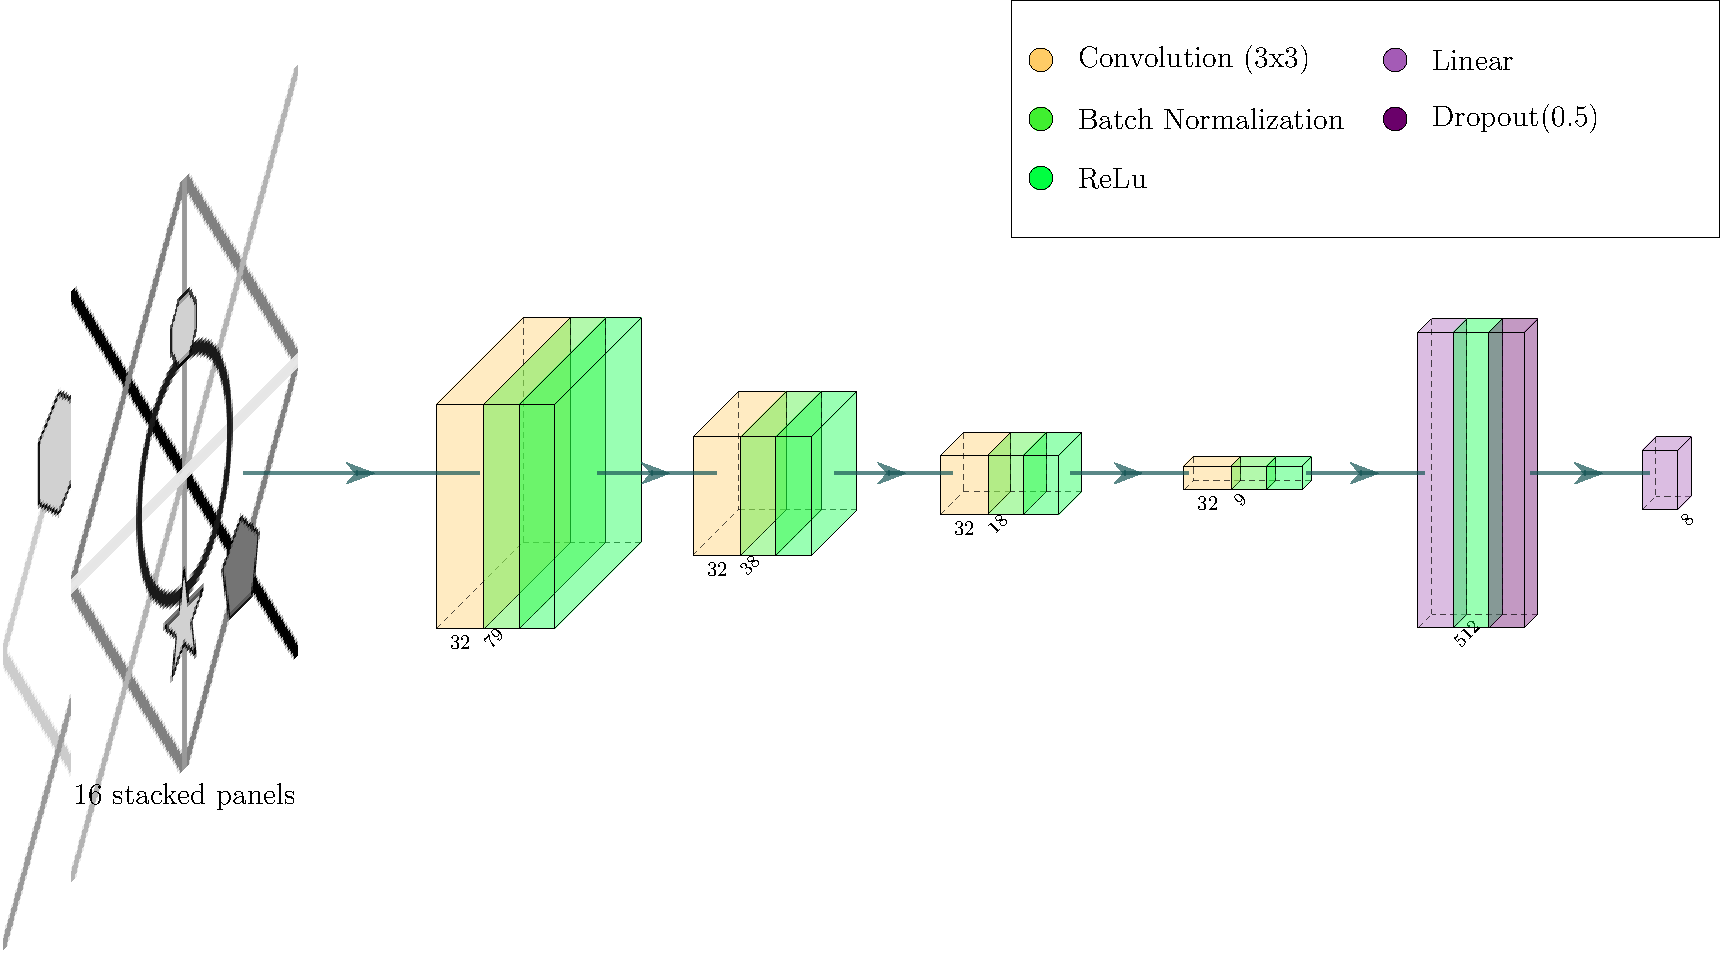
\includegraphics[width=\textwidth]{arhitekture/cnn.pdf}
    \caption{Графички приказ конволуционе мреже са потпуно повезаним слојевима}
    \label{fig:cnnmlp}
\end{figure}

\subsection{Конволуциона мрежа са ДКМ блоковима}

Архитектура конволуционе неуралне мреже са ДКМ блоковима је преузета из рада \cite{barrett_measuring_2018}.
Број филтара је 8 из разлога што се у овом случају конволуција примењује на сваку слику посебно и самим тим је потребана мања величин латентног вектора.
Остали параметри КНН су непромењени у односу на претходну архитектуру. 
Величина скривеног слоја, односно величина сигнала за краткорочну и сигнала за дугорочну меморију је је 96.
Табеларни приказ архитектуре је 
приказан на табели \ref{tab:cnnlstm} , а графички приказ на слици \ref{fig:cnnlstm}.

\begin{table}[h]
    \centering
    \begin{tabular}{l | c}
    \hline
    Назив хипер-параметра & Вредност\\
    \hline
        КНН - број филтара & [8, 8, 8, 8]\\
        КНН - померај филтра & 2\\
        КНН - величина филтра & 3x3\\
        КДМ - скривени слој & 96\\
        Pроценат изостављања & 0.5
    \end{tabular}
    \caption{Табеларни приказ хипер-параметара мреже}
    \label{tab:cnnlstm}
\end{table}

\begin{figure}[h]
    \centering
    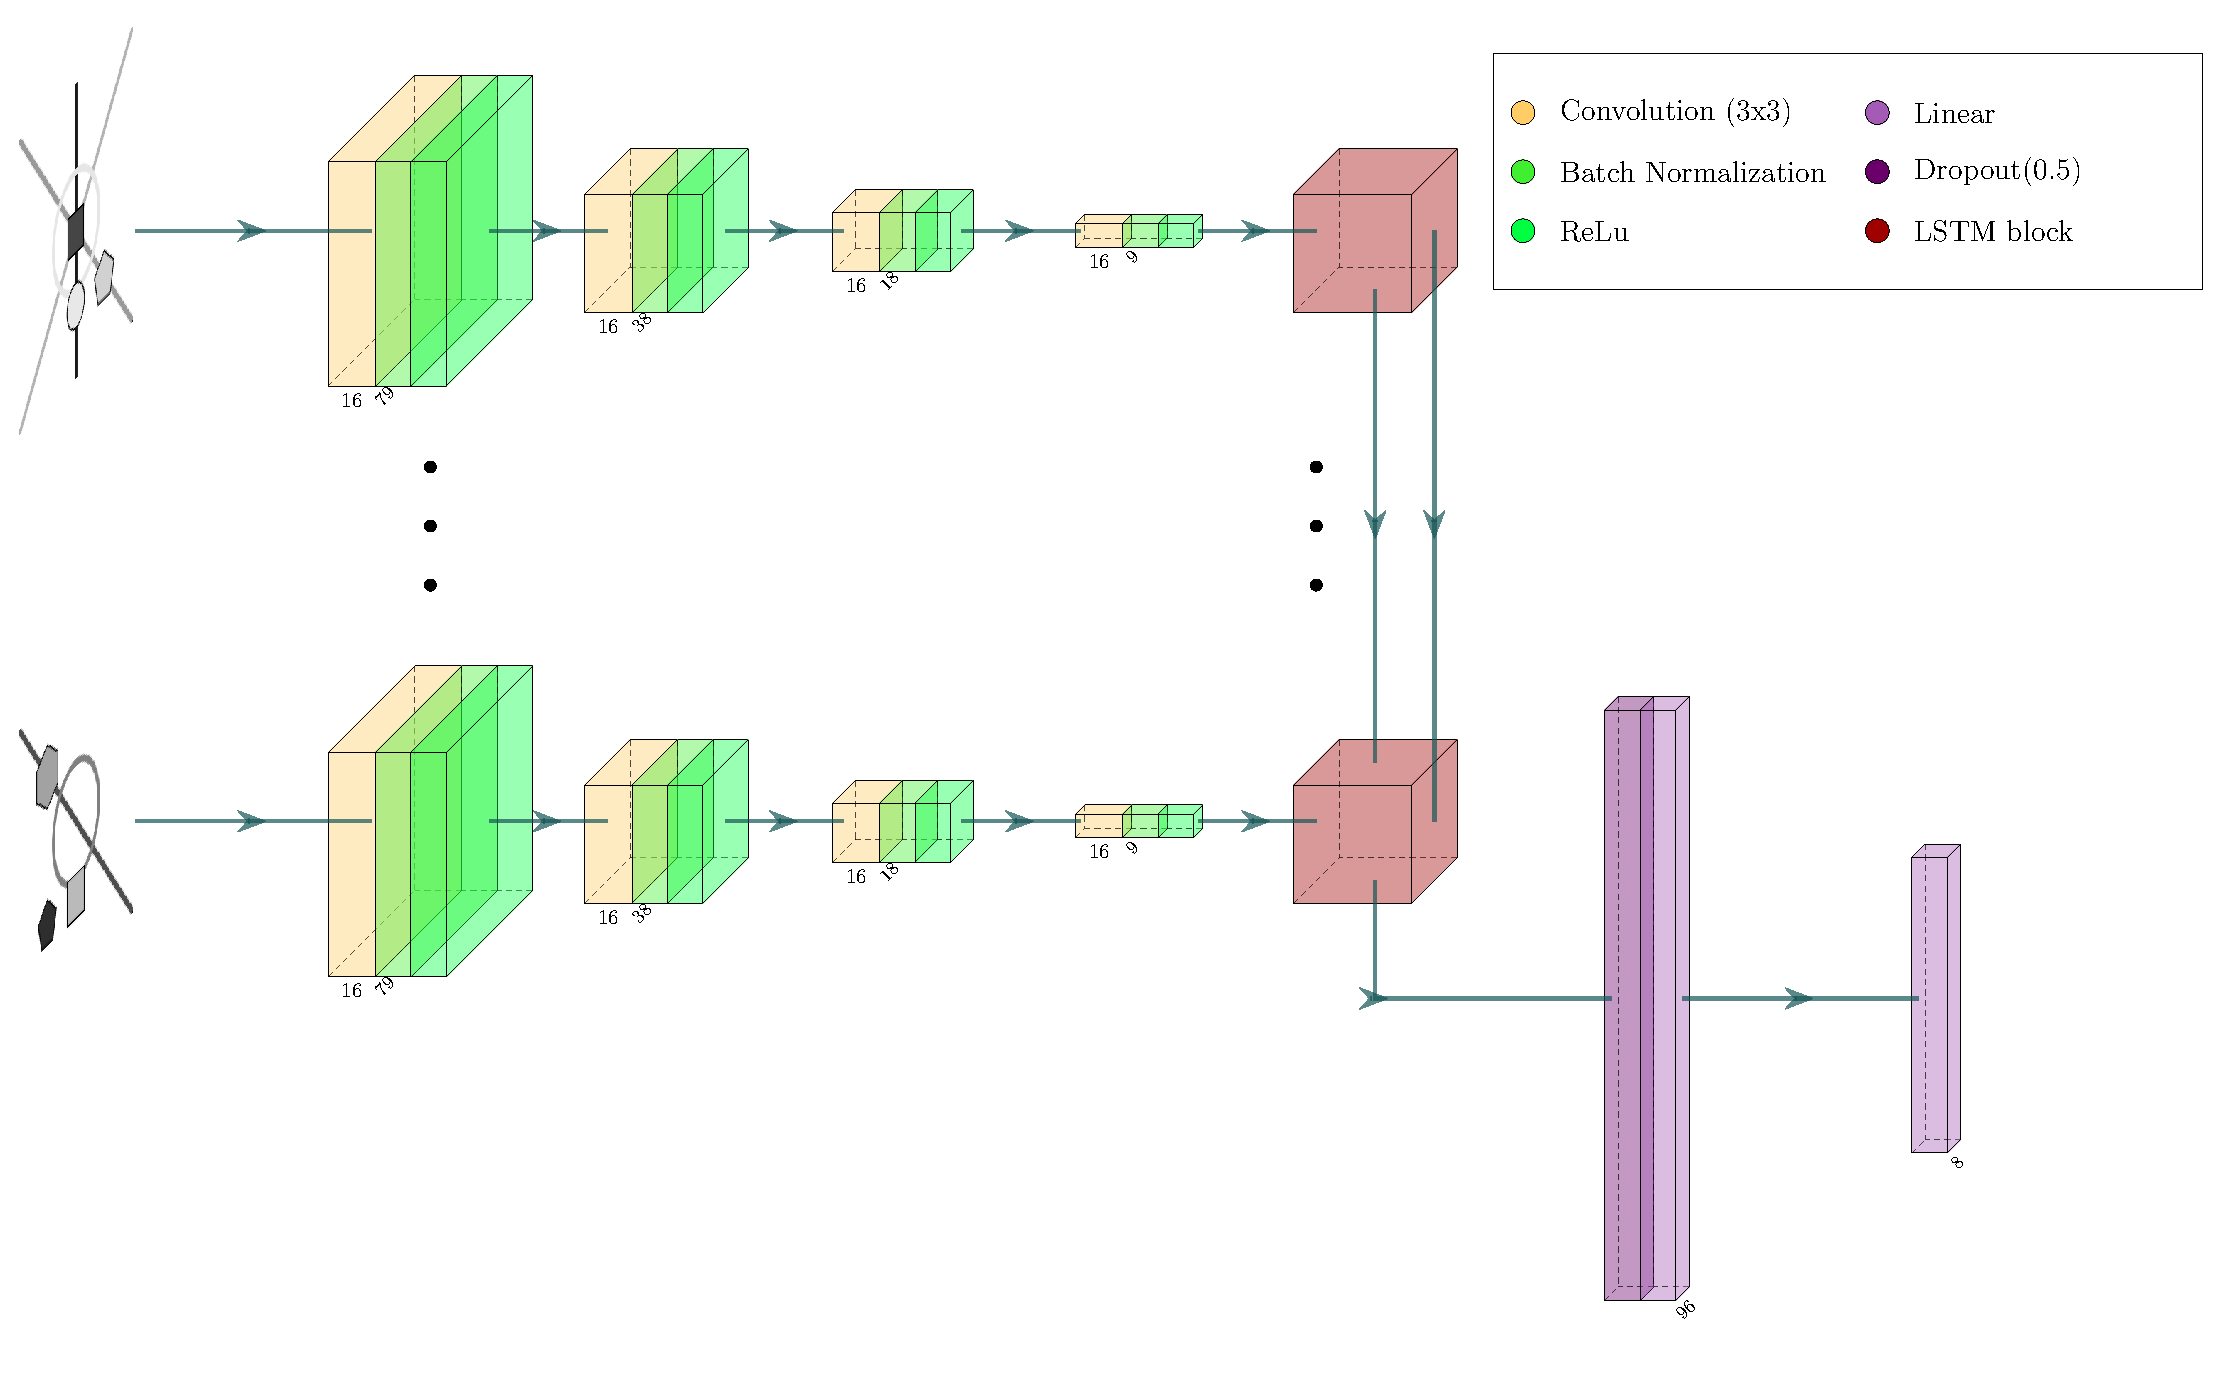
\includegraphics[width=\textwidth]{arhitekture/cnn_lstm.pdf}
    \caption{Графички приказ конволуционе мреже КДМ блоковима}
    \label{fig:cnnlstm}
\end{figure}

\subsection{Конволуциона мрежа са РНН}
Главни допринос рада \cite{barrett_measuring_2018} јесте увођење нове архитектуре за решавање Рејвенових матрица. Они су представили 
нову архитектуру рекурентних неуралних мрежа за решавање Рејвенових тестова(Wild Relation Neural Network - WREN) по презимену једног од аутора (Wild).
За потребе овог рада је прузета њихова архитектура, са изменама у слоју Ф. У референтом раду су користили додатне информације у виду мета матрица како би побоњшали перформансе модела. 
Пошто се у овом раду бавимо само простом класификацијом, уместо 13 излаза, наша архитектура има само 1 који представља резултат колико се потенцијални одговор уклапа у контекст.
\newline

Први део архитектуре чини конволуциони слој који се примењује на све слике из теста појединачно \ref{fig:wren1}, а затим се на латентни вектор додаје ознака која је слика у питању. 
За потребе означавања се додаје \textit{one hot} вектор на латентни вектор сваке од слика. На крају се означени вектор пропушта кроз потпуно повезани слој са једним слојем како би векторска представа слике била одређене величине.
\newline

\begin{figure}[H]
    \centering
    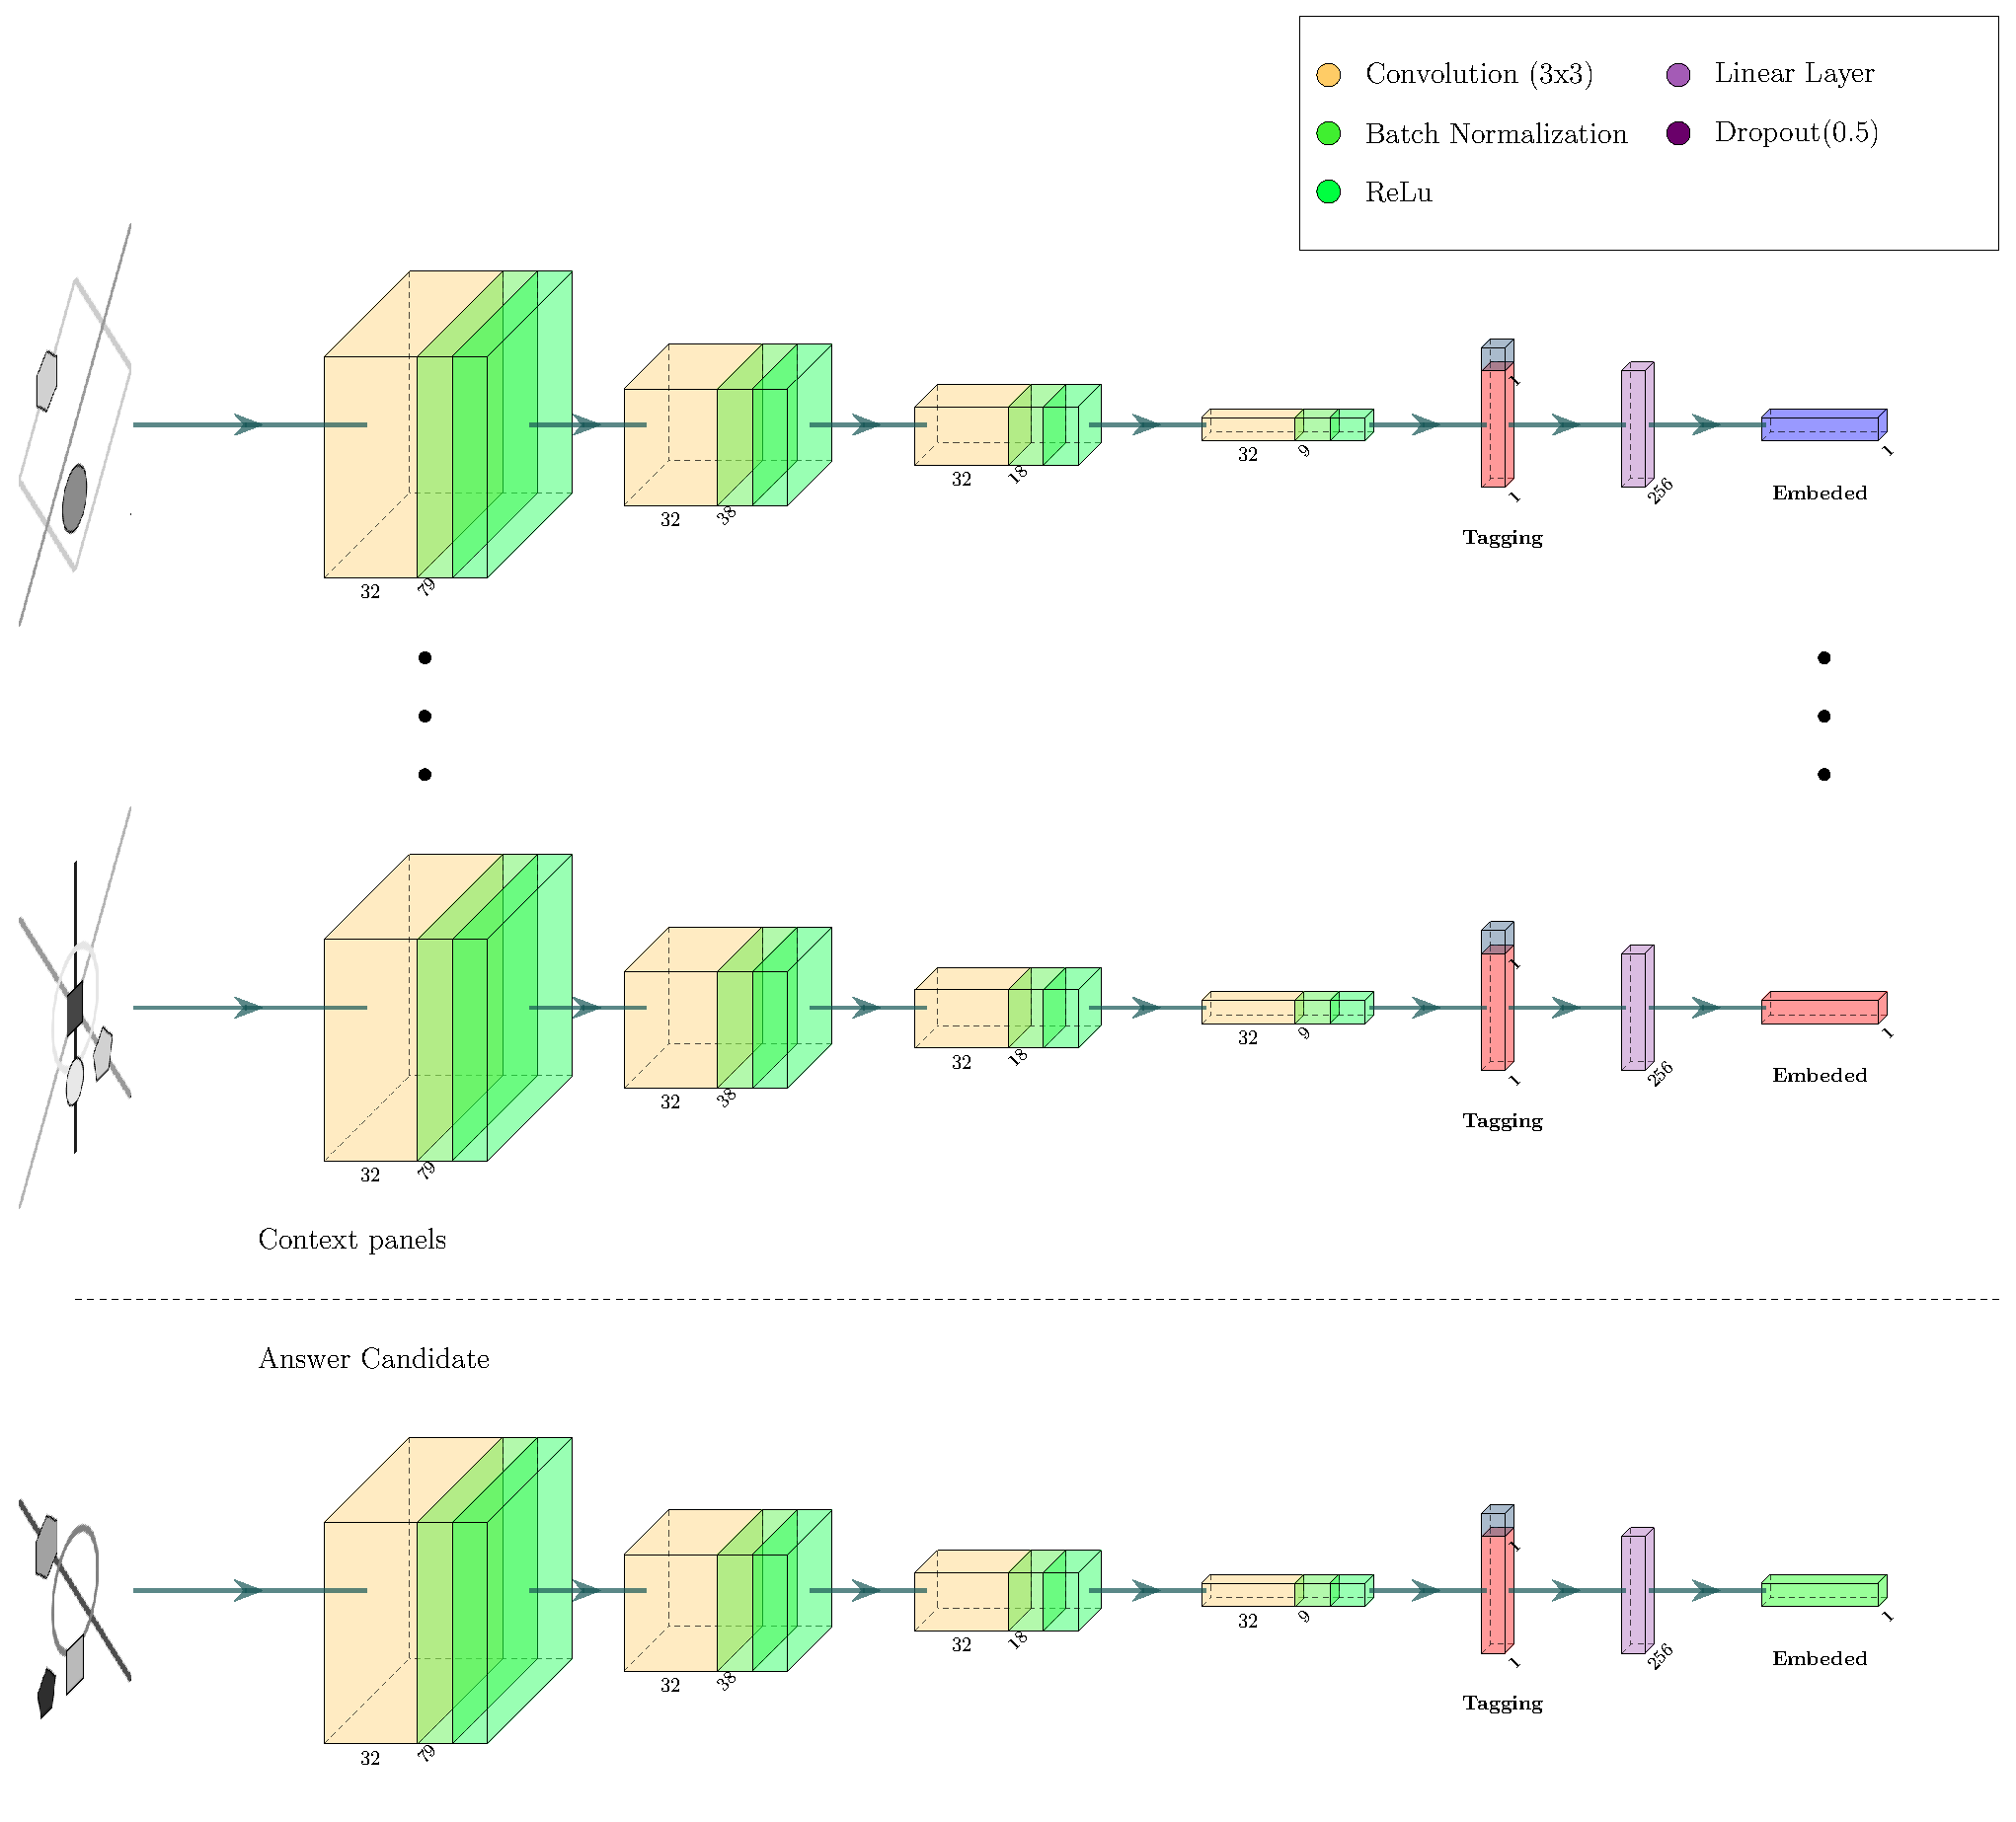
\includegraphics[width=\textwidth]{arhitekture/wren1.pdf}
    \caption{Графички приказ првог дела WREN архитектуре}
    \label{fig:wren1}
\end{figure}

Након што је припремљена векторска репрезетација, подаци се пропуштају кроз РНН - спајају се све могуће варијације вектора контексних панела са једним вектором из потенцијалних одговора. Ово се ради појединачно за сваки потенцијални одговор. 
Спојени вектори пропуштају кроз потпуно повезану неуралну мрежу Г \ref{fig:wren2}. Након тога се сви резултати за један потенцијални одговор сабирају.
Збир се пропушта кроз Потпуно повезани слој Ф. Резултат овог дела архитектуре је једна вредност за сваки потенцијални одговор која представња његов резултат уклапања. 
\newline

\begin{figure}[H]
    \centering
    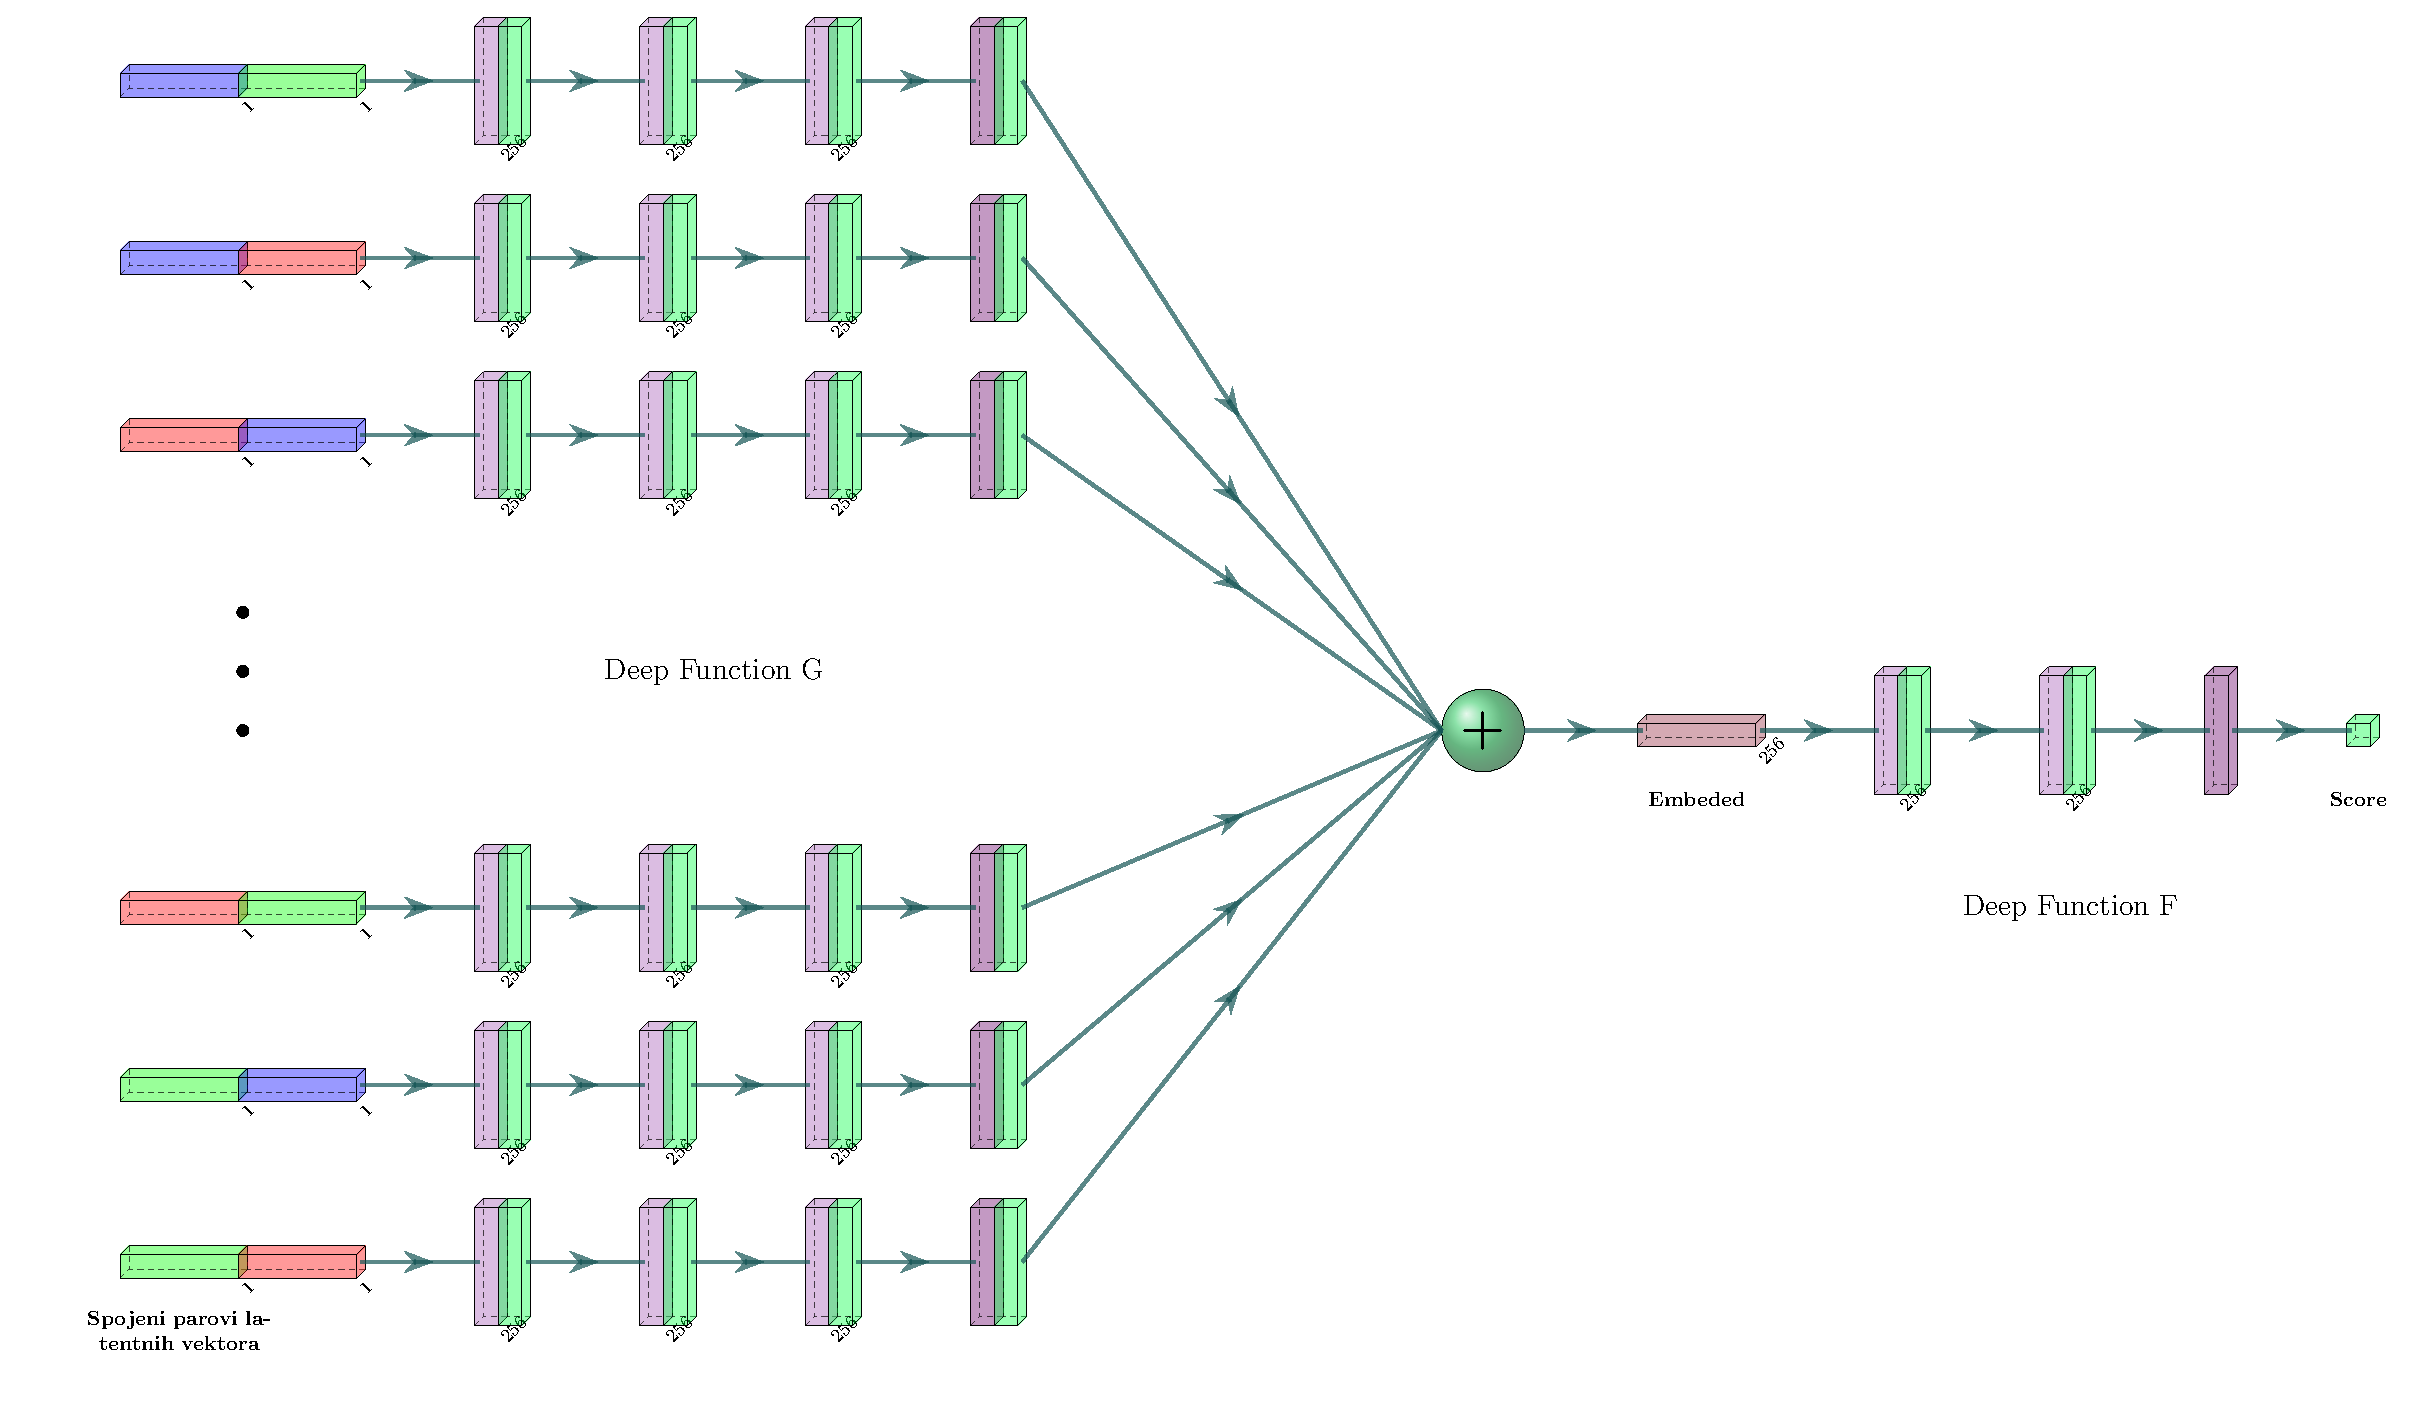
\includegraphics[width=\textwidth]{arhitekture/wren2.pdf}
    \caption{Графички приказ другог дела WREN архитектуре}
    \label{fig:wren2}
\end{figure}

На крају, се резултати спајају у један вектор и примењује софмакс функција. Резултат је вектор који садржи вероватноће да је понуђени одговор прави. Након тога се одређује индекс одговора са највећом вероватноћом што представња коначан излаз мреже - argmax.
\newline

\begin{figure}[H]
    \centering
    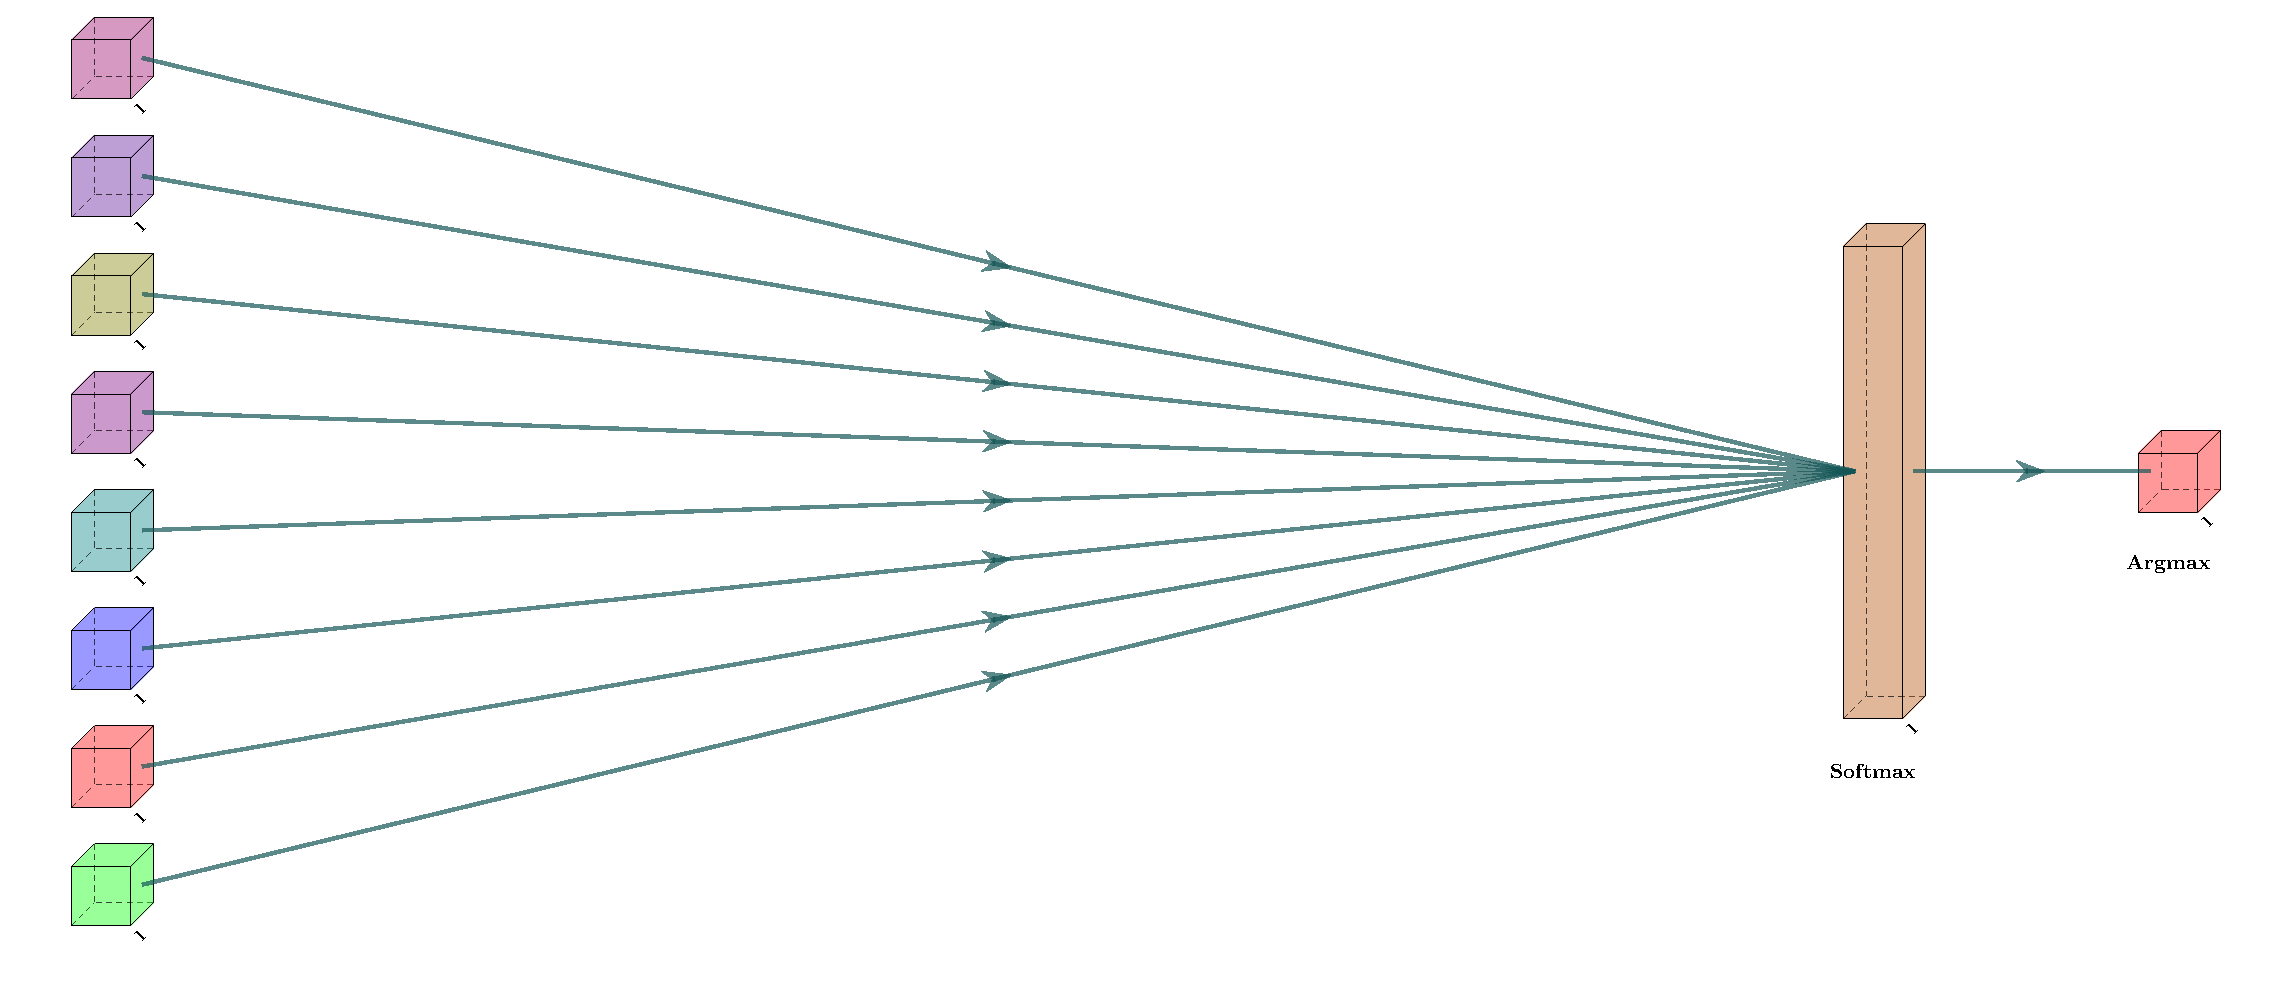
\includegraphics[width=\textwidth]{arhitekture/wren3.pdf}
    \caption{Графички приказ трећег дела WREN архитектуре}
    \label{fig:wren3}
\end{figure}

Табеларни приказ хипер-параметара архитектуре је приказан у табели \ref{tab:wren}

\begin{table}[H]
    \centering
    \begin{tabular}{l | c}
    \hline
    Назив хипер-параметра & Вредност\\
    \hline
        КНМ - број филтара & [32, 32, 32, 32]\\
        КНМ - померај филтра & 2\\
        КНМ - величина филтра & 3x3\\
        Слој за енкодовање & 256\\
        ППНМ - Г & [256, 256, 256, 256]\\
        ППНМ - Ф енкодовање & [256, 256, 1]\\
        Pроценат изостављања & 0.5
    \end{tabular}
    \caption{Табеларни приказ хипер-параметара мреже}
    \label{tab:wren}
\end{table}


\section{Архитектурa софтвера}
\label{sec:41}

Због чињенице да све три описане архитектуре имају исти улаз и исти излаз, могуће је издвојити логику за тренинг и рачунање губитка у апстрактну класу \textit{BaseModel} која поседује апстрактну функцију \textit{forward}. 
Остале класе које дефинишу различите архитектуре наслешују све функционалности \textit{BaseModel} касе, графички приказ је приложен на слици \ref{fig:klase}.

\begin{figure}[H]
    \centering
    \resizebox{0.7\textwidth}{!}{%
    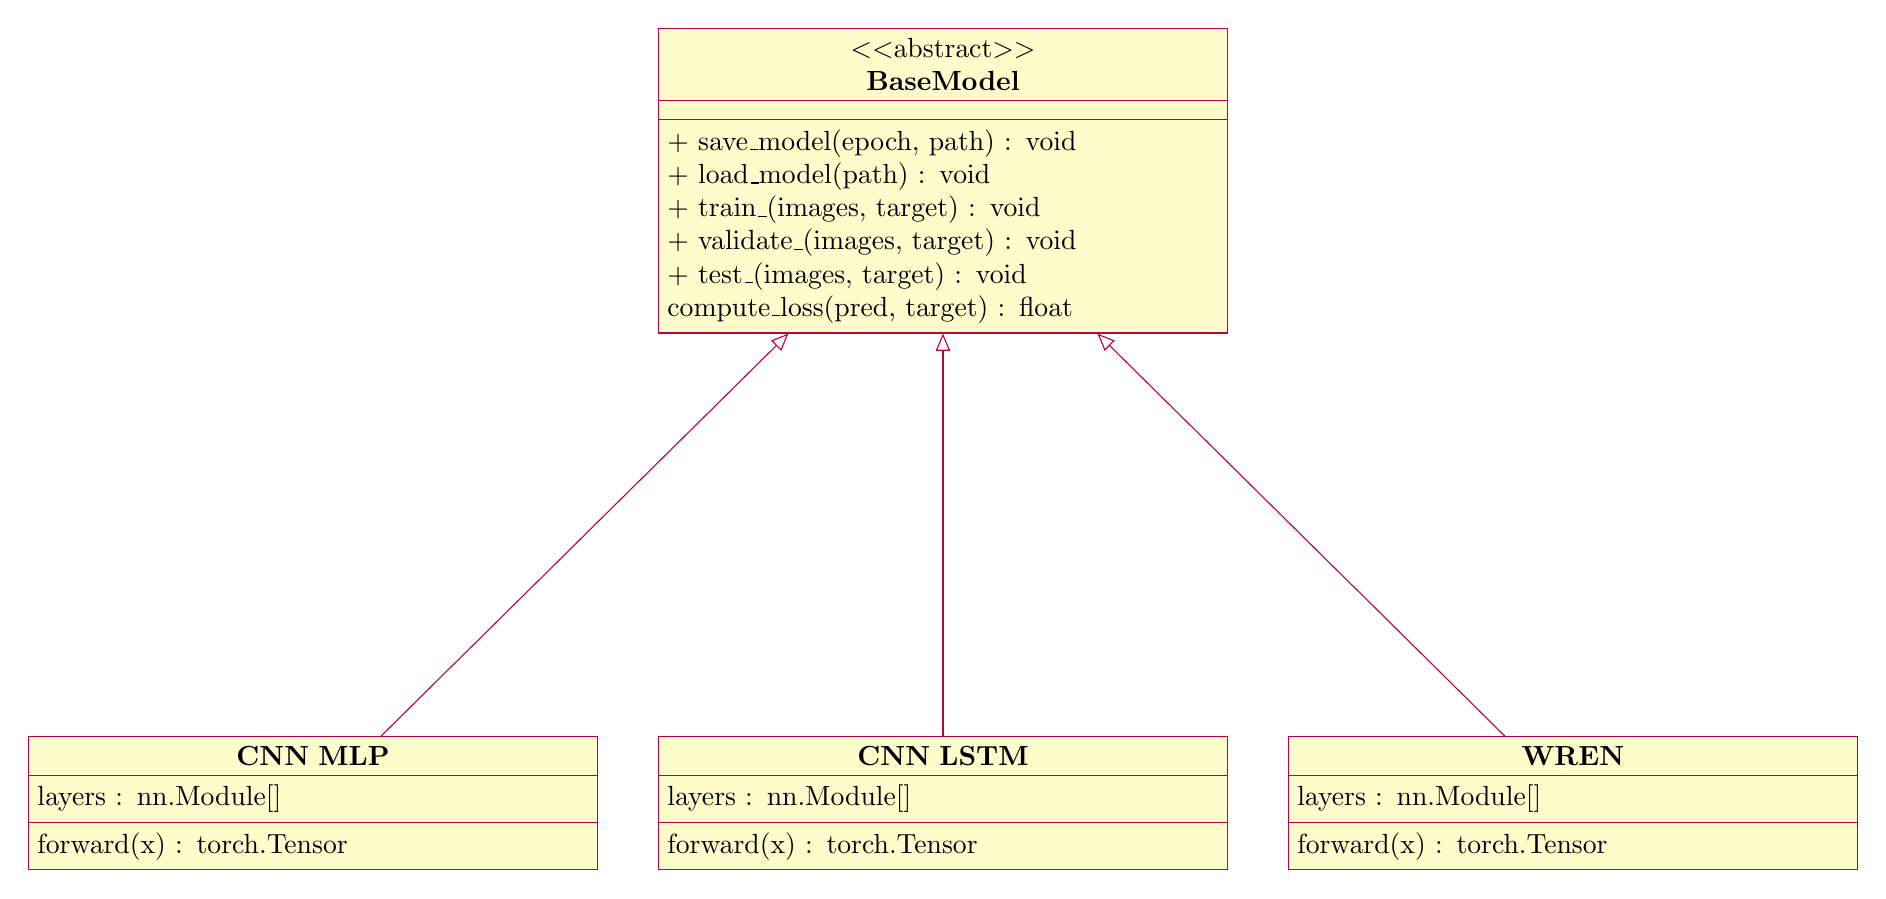
\begin{tikzpicture}
        \begin{abstractclass}[text width=7cm]{BaseModel}{0,0}
            \operation{+ save\_model(epoch, path) : void}
            \operation{+ load\_model(path) : void}
            \operation{+ train\_(images, target) : void}
            \operation{+ validate\_(images, target) : void}
            \operation{+ test\_(images, target) : void}
            \operation{compute\_loss(pred, target) : float}
          \end{abstractclass}
        
          \begin{class}[text width=7cm]{CNN MLP}{-8,-9}
            \inherit{BaseModel}
            \attribute{layers : nn.Module[]}
            \operation{forward(x) : torch.Tensor}
            
          \end{class}

          \begin{class}[text width=7cm]{CNN LSTM}{0,-9}
            \inherit{BaseModel}
            \attribute{layers : nn.Module[]}
            \operation{forward(x) : torch.Tensor}
          \end{class}

          \begin{class}[text width=7cm]{WREN}{8,-9}
            \inherit{BaseModel}
            \attribute{layers : nn.Module[]}
            \operation{forward(x) : torch.Tensor}
          \end{class}
    \end{tikzpicture}
}
    \caption{Графички приказ функције активације исправљача}
    \label{fig:klase}
\end{figure}

\subsubsection{Основни (базни) модел}

Основни базни модел имплементира основну логику тренирања модела. Прво се градијенти поставе на 0, затим се тренинг подаци провуку кроз мрежу након чега се израчуна функција грешке. 
На основу функције грешке се ажурирају тежине, а функција враћа колика је вредност функције губитка као и колико је примера тачно урађено у тренутној гомили.
Алгоритам који је имплементиран за тренинг је приказан 
у псеудо коду \ref{alg3}.

Алгоритми за валидацију и тестирање не поседују кораке за ажурирање тежине, него само за предикцију и број тачно урађених тестова у итерацији.


\begin{algorithm}[h]
    \caption{Алгоритам једне итерације тренинга}
    \label{alg3}
    \begin{algorithmic}[1]
    \Procedure{train\_}{$input, target$}
        \State $ reset\_gradients()$
        \State $output \gets forward(input)$
        \State $loss \gets compute\_loss(output, target)$
        \State $loss.backward()$
        \State $update\_weights()$
        \State $pred \gets argmax(output)$
        \State $correct \gets count_matching\_elements(pred, target)$
        \State \Return $loss, correct size(target)$
    \EndProcedure
    \end{algorithmic}
    \end{algorithm}

\subsubsection{Модел конволуционе мреже са потпуно повезаним слојевима} 
За имплементацију модела конволуционе мреже са потпуно повезаним слојевима су коришћене готове класе библиотеке 
\textit{Torch}: \textit{Conv2d} i \textit{Linear}. Оне су иницијализоване са параметрима описаним у табели \ref{tab:cnnmlp}.

Додатно после сваке конволуције је примењена нормализација хрпе у конволуционом слоју, ППНМ је имплементирано изоставњање у претпоследњем слоју.

\subsubsection{Модел конволуционе мреже са ДКМ ћелијама}
Поред модула описаних у претходној секцији, у сврху моделирања конволуционе мреже са ДКМ ћелијама је искоришћена класа \textit{LSTM} из истог модула.
Сви параметри су презети из табеле \ref{tab:cnnlstm}.

\subsubsection{Модел конволуционе мреже са релационим слојевима}

Модул за РНН је имплементиран помоћу интерфејса за креирање слојева \textit{torch.nn.Module}. 
Комбиновање латентих вектора је урађено проширивањем димензија оргиналног тенсора. Прво се проширила претпоследња димензија чиме
је добијен тенсор којем се у претпоследњој димензији сваки латентни вектор понавња узастопно N пута, затим је проширивање урађено 
по трећој димензији са краја чиме смо добили тенсор којем се у последњљм слоју наизменично понавњају вектори N пута. Када спојимо 
ова два тенсора резултат је тенсор са свим могућим варијацијама скупа латентних вектора.

Приликом ове операције градијенти се клонирају, а приликом проласка уназад се гледа просек градијената копија при рачунању следећег градијента у ланцу.

\section{Функција губитка, оптимизатор и учитавање података}
\label{sec:43}

За функцију губитка је изабрана унакрсна ентропија из одењка \ref{sec:261}. Она је имплементирана у библиотеци под именом \textit{cross\_entropy()}.
\newline

Адам је изабран као оптимизатор модела са парамтерима приказаним у табели \ref{tab:adam}:

\begin{table}[H]
    \centering
    \begin{tabular}{l | c}
    \hline
    Параметар & Вредност\\
    \hline
        $learning\_rate$ & 0.0003\\
        $\beta1$ & 0.9\\
        $\beta2$ & 0.999\\
        $\epsilon$ & $1^{-8}$\\
    \end{tabular}
    \caption{Табеларни приказ апраметара Адам оптимизатора}
    \label{tab:adam}
\end{table}



\chapter{Резултати и дискусија}
\label{sec:5}

У овом поглављу прво ће бити описан хардвер на коме су резултати добијени, 
затим софтверски стек (енг. \textit{software stack}) који је коришћен при 
обучавању и тестирању модела како би се отклониле евентуалне системске зависности. Потом, 
биће представљени и резултати овог рада у виду више решења проблема, свако са 
својим каратеристикама. Финално, биће дискутоване разике између решења и њихова могућа побољшања.

\section{Тест платформа}
\label{sec:51}

За потребе овога рада је коришћен рачунарски сервер са хардверским акцелератором са ознаком \textit{NVIDIA GeForce RTX 3060} и меморијским капацитетом од 12GB.
Берзије драјвера и \textit{CUDA toolkit}-a је приложен у табели \ref{tab:hw}.
\newline

\begin{table}[h]
    \centering
    \begin{tabular}{l | c}
    \hline
    Назив & Верзија\\
    \hline
        Driver & 530.30.02\\
        CUDA & 12.1 \\
    \end{tabular}
    \caption{Верзије драјвера и \textit{toolkit-a}}
    \label{tab:hw}
\end{table}

При изради софтверског решења су искоришћене верзије програма и бибилиотека који се могу видети у табели \ref{tab:sw}:
\newline

\begin{table}[h]
    \centering
    \begin{tabular}{l | c}
    \hline
    Назив програма или библиотеке & Верзија\\
    \hline
        Python3 & 3.10.12\\
        torch & 2.0.1\\
        torchvision & 0.15.2\\
        tqdm & 4.66.1\\
        matplotlib & 3.7.2
    \end{tabular}
    \caption{Верзије софтера и библиотека у ком је израђен софтверски део решења}
    \label{tab:sw}
\end{table}

\section{Методологија тестирања}
\label{sec:52}

Сви модели су обучавани на истом тренинг и валидационом скупу. Параметри оптимизатора су приказани у табели \ref{tab:adam}, са гомилама величине 32 (енг. \textit{batch\_size}).
Због величине скупа података за тренирање валидација је вршена на сваких 10\% обраћених података.
У свим случајевима обучавања је имплементиран механизам раног заустављања (енг. \textit{early\_stopping}). Критеријум за рано зауставњање је да се после треће епохе не повећа 
тачност на три узастопна валидациона сета на крају епохе.
\newline

После сваке епохе се чувају параметри модела, а приликом тестирања се користи модел који је имао највећу прецизност на валидационом скупу.
\newline

Максимална вредност епохе је 16.
\newline

Све слике су смањене на димензије 80х80 коришћењем интерполације најближих суседа.
\newline

\section{Резултати и дискусија}
\label{sec:53}


\subsection{Обучавање модела}

\subsubsection{Модел конволуционе мреже са потпуно повезаним слојевима}

На слици \ref{fig:mlpacc} је приказана кумулативна прецизност модела по хрпи током тренирања. Примећујемо да 
је прецизност на валидационом и тренинг скупу прате једна другу што говори да није дошло до преобучавања. 
Приметно да се прецизност повећава током обуке, али није достигла плато, односно максималну вредност што говори да би модел постигао још већу прецизност
при повећању броја епоха.
\newline

\begin{figure}[H]
    \centering
    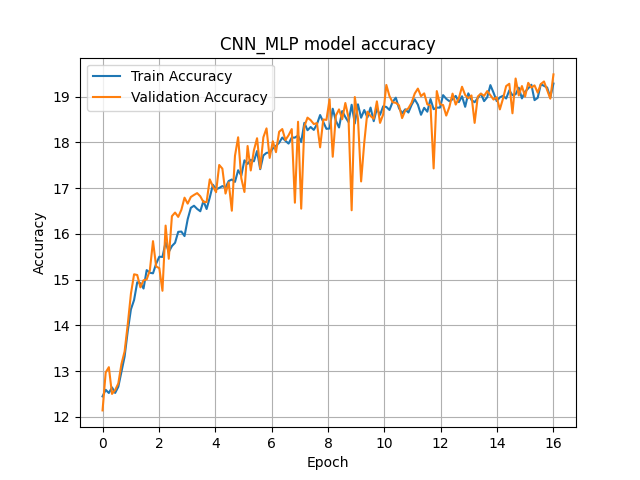
\includegraphics[width=0.7\textwidth]{../Results/CNN_MLP_19_09_09/accuracy.png}
    \caption{Графички приказ првог дела WREN архитектуре}
    \label{fig:mlpacc}
\end{figure}


\subsubsection{Модел конволуционе мреже са КДМ ћелијама}

На слици \ref{fig:mlpacc} је приказана кумулативна прецизност модела по хрпи током тренирања. Примећујемо благо раздвајање у кривама после шесте епохе, што говори да је дошло до благог преобучавања. 

Као што је случај код претходног модела, и овде је приметно да крива није сдостигла свој максимум. Али је у односу на претходни случај степен раста мањи у односу на претходни модел што 
имплицира да овај модел брже конвергира оптималним праметрима од претходног модела за параметре прослеђене оптимизатору.
\newline

\begin{figure}[H]
    \centering
    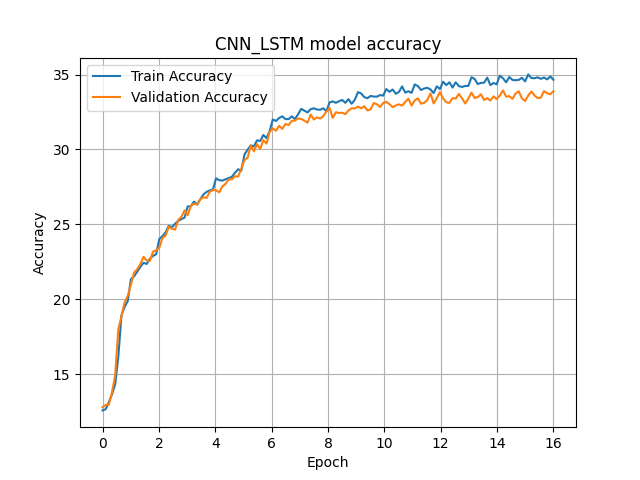
\includegraphics[width=0.7\textwidth]{../Results/CNN_LSTM_21_11_09/accuracy.png}
    \caption{Графички приказ првог дела WREN архитектуре}
    \label{fig:mlpacc}
\end{figure}

\subsubsection{Модел конволуционе мреже са РНН}

На слици \ref{fig:mlpacc} одмах уочавамо да се десило рано заустављање после десете епохе. Евидентно да је дошло до преобучавања модела.
Крива тачности на тесту за валидацију је изломњена и нема тенденцију раста.

\begin{figure}[H]
    \centering
    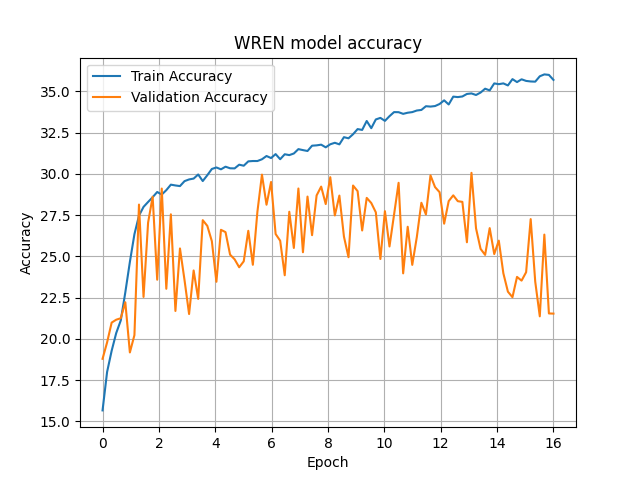
\includegraphics[width=0.7\textwidth]{../Results/WildRelationalNetwork_22_17_09/accuracy.png}
    \caption{Графички приказ првог дела WREN архитектуре}
    \label{fig:mlpacc}
\end{figure}

\subsection{Резултати}

У табели \ref{tab:pr} је приказана прецизност модела на скупу за тестирање. 
Најмању прецизност је постигла конволуциона неурална мрежа са потпуно потпуно повезаним слојем од $19.2 \%$ што је и било очекивано с обзиром 
да је мрежа са најмање параметара и није показано да овакав тип неуронских мрежа успешно препознаје релације.
Најбољи резултат је постигла неурална мрежа са дугорошно-краткорочним меоријским ћелијама са прецизношћу од $33.9 \%$. 
Модел са рекурентном нуронском мрежом је постигао прецизност од $28.2 \%$ што је испод вредности коју су добили у раду \cite{barrett_measuring_2018}.
Ово одступање може бити објашњено што у овом раду није примењено додатно обучавање мета подацима.
\newline

\begin{table}[h]
    \centering
    \begin{tabular}{l | c}
    \hline
    Модел & Прецизност [\%]\\
    \hline
        КНН + ППНМ &$ 19.2$\\
        КНН + ДКМ & $ 33.9$\\
        КНН + РНМ & $28.2 $\\
    \end{tabular}
    \caption{Приказ прецизности по моделу}
    \label{tab:pr}
\end{table}

Све три мреже су постигле тачност већу од случајног одабира на довољно великом скупу података. Можемо рећи да су сви модели у некој мери научени да решавају Рејвенове тестове.
На основу тачности током обучавања можемо закључити да прва два модела потенцијално могу постићи боље резултате ако би се обучавале у већем броју епоха.
Модел са рекурентним слојем се преобучио, што показује да мрежа има могућност решавања тестова, али ”на памет”. Дефинитивно је показала потенцијал у домену решавања Рејвенових тестова, али 
је потребно додатно испитивање хипер параметара како би се креирала архитектура која има већу моћ генерализације.

\chapter{Закључак }
\label{sec:6}

Овај рад је увео питање да ли неуронске мреже поседују способност апстрактног резоновања. Пројектоване су три суштински различите архитектуре неуронских мрежа како би се кроз што већи број
примера покушао пронаћи одговор на ово питање. Сви модели су постигли резултате који су већи од случајне вредности што је добар показатељ да модели у одређеној мери разумеју како да реше Рејвенове тестове.
Поставња се питање како би се просечан човек снашао у решавању ове врсте тестова и да ли би постигао боље резултате на скупу за тестирање. 
\newline

Показало се да генерални модели као што је конволуциона неурална мрежа са поптпуно повезаним слојем значајно лошије решавала тестове од осталих модела. Потребно је посебно моделовање неуронских мрежа које разумеју релације и прогресије 
како би се прецизност увећала. Иако неуронске мреже у одређеној мери имају могућност апстрактног резоновања кључну улогу игра њихово пројектовање и хипер параметри.
\newline

И даље остаје отворено питање да ли долази до појаве апстрактног резоновања уколико је човек или машина учила да решава одређену врсту тестова. Јер, иако су подаци за тест и тренинг одвојени они суштински представљају исту класу проблема.
\newline

Чињеница да се модел са релационим слојем преобучио показује да се треба посветити додатна пажња проучавању овог типа архитектуре и да она има потенцијал. Потребно је урадити опширнију анализу хипер параметара. Такође је потребно
повећати број епоха тренирања и конструисати адекватније параметре оптимизатора како би ови модели брже конвергирали.

%\chapter{Литература}
%\label{sec:7}

% Predlažem upotrebu bibtex i kreiranje .bib fajlova, a da se podaci za njh skidaju sa Google Scholar i sličnih servisa
\bibliographystyle{ieeetr}
\bibliography{diplomski.bib}
%\addcontentsline{toc}{chapter}{Литература}

% Alternativni način
%\begin{thebibliography}{10}
%\bibitem{Shalev-Shwartz:2014:UML:2621980}
%S. Shalev-Shwartz, S. Ben-David, \emph{Understanding MachineLearning}, Cambridge, 2016
%\end{thebibliography}

\end{document}